% !TeX TXS-program:compile = txs:///pdflatex/[--shell-escape]
\documentclass[13pt,landscape,a4paper]{article}
\usepackage[normalem]{ulem}
\usepackage{tikz}
\usetikzlibrary{shapes,positioning,arrows,fit,calc,graphs,graphs.standard}
\usepackage[nosf]{kpfonts}
\usepackage[t1]{sourcesanspro}
\usepackage{multicol}
\usepackage{wrapfig}
\usepackage[top=1mm,bottom=1mm,left=1mm,right=1mm]{geometry}
\usepackage[framemethod=tikz]{mdframed}
\usepackage{microtype}
\usepackage{tabularx}
\usepackage{hhline}
\usepackage{makecell}
\usepackage{mathtools}
\usepackage{subfig}
\usepackage{listings}

\DeclarePairedDelimiter{\ceil}{\lceil}{\rceil}

\newcommand\codeblue[1]{\textcolor{blue}{\code{#1}}}
\newcommand\ctrimg[2][0.8]{\begin{center}\includegraphics[width=#1\columnwidth]{#2} \end{center}}
\newcommand\red[1]{\textcolor{red}{#1}}

\usepackage{lastpage}
\usepackage{datetime}
\yyyymmdddate
\renewcommand{\dateseparator}{-}
\let\bar\overline

\definecolor{myblue}{cmyk}{1,.72,0,.38}

\def\firstcircle{(0,0) circle (1.5cm)}
\def\secondcircle{(0:2cm) circle (1.5cm)}

\colorlet{circle edge}{myblue}
\colorlet{circle area}{myblue!5}

\tikzset{filled/.style={fill=circle area, draw=circle edge, thick},
    outline/.style={draw=circle edge, thick}}

\pgfdeclarelayer{background}
\pgfsetlayers{background,main}

\renewcommand{\baselinestretch}{.8}
\pagestyle{empty}

\global\mdfdefinestyle{header}{%
    linecolor=gray,linewidth=1pt,%
    leftmargin=0mm,rightmargin=0mm,skipbelow=0mm,skipabove=0mm,
}

\let\counterwithout\relax
\let\counterwithin\relax
\usepackage{chngcntr}
\usepackage{verbatim}
\usepackage{etoolbox}
\makeatletter
\preto{\@verbatim}{\topsep=0pt \partopsep=0pt }
\makeatother

\counterwithin*{equation}{section}
\counterwithin*{equation}{subsection}
\usepackage{enumitem}
\newlist{legal}{enumerate}{10}
\setlist[legal]{label*=\arabic*.,leftmargin=2.5mm}
\setlist[itemize]{leftmargin=4mm}
\setlist[enumerate]{leftmargin=4.5mm}
\setlist{nosep}
\usepackage{minted}

\def\code#1{\texttt{#1}}

\newenvironment{descitemize} % a mixture of description and itemize
{\begin{description}[leftmargin=*,before=\let\makelabel\descitemlabel]}
    {\end{description}}

\newcommand{\descitemlabel}[1]{%
    \textbullet\ \textbf{#1}%
}
\makeatletter

\renewcommand{\section}{\@startsection{section}{1}{0mm}%
    {.2ex}%
    {.2ex}%x
    {\color{myblue}\sffamily\small\bfseries}}
\renewcommand{\subsection}{\@startsection{subsection}{1}{0mm}%
    {.2ex}%
    {.2ex}%x
    {\sffamily\bfseries}}
\renewcommand{\subsubsection}{\@startsection{subsubsection}{1}{0mm}%
    {.2ex}%
    {.2ex}%x
    {\rmfamily\bfseries}}

\def\mathcolor#1#{\@mathcolor{#1}}
\def\@mathcolor#1#2#3{%
    \protect\leavevmode
    \begingroup
    \color#1{#2}#3%
    \endgroup
}

\makeatother
\setlength{\parindent}{0pt}

\setminted{tabsize=2, breaklines}
% Remove belowskip of minted
\setlength\partopsep{-\topsep}

\newcolumntype{a}{>{\hsize=1.5\hsize}X}
\newcolumntype{b}{>{\hsize=.25\hsize}X}

\setlength\columnsep{1.5pt}
\setlength\columnseprule{0.1pt}
\begin{document}
    \setlength{\abovedisplayskip}{0pt}
    \setlength{\belowdisplayskip}{0pt}

    \scriptsize
    \begin{multicols*}{3}
        \raggedcolumns
        \section{Introduction to OS}
        \subsection{What is OS?}
        \begin{itemize}
            \item A program that acts as an \textbf{intermediary} between a computer user and the computer hardware (allows user programs to interact with hardware in a safe way)
            \item Manages hardware and software resources and provides essential services to other programs
        \end{itemize}
        \subsection{Brief History of OS}
        OS evolves with:
        \begin{itemize}
            \item Computer Hardware (e.g. integration of GPU, Multicore CPU)
            \item User application and usage patterns (e.g. phones have different UI than computers)
        \end{itemize}
        \subsubsection{OS for the first computers}
        \begin{enumerate}
            \item \textbf{No OS}
            \begin{itemize}
                \item Programs directly interacted with hardware
                \item \textbf{Advantage}: Minimal Overhead
                \item \textbf{Disadvantages}: Not portable, inflexible and does not use computer resources efficiently
            \end{itemize}
            \item \textbf{Batch OS}
            \begin{itemize}
                \item Allows for batch processing but programs by storing programs as digital format (e.g. tapes)
                \item As a user, you still interact directly with the hardware, with additional information for the OS (resources required, job specification)
                \item \textbf{Advantage}: Batch processing (write multiple programs and leave it to run)
                \item \textbf{Disadvantages}: Inefficient (CPU idle when performing I/O)
            \end{itemize}
            \item \textbf{Time-sharing OS}\\
            \textbf{Time sharing}: Multiple users running multiple programs, \textbf{Multiprogramming}: 1 user running multiple programs (To have time sharing, we must have multiprogramming)
            \begin{itemize}
                \item Allows multiple users to interact with machines using terminals
                \item supports Job scheduling $\rightarrow$ concurrency of programs
                \item \textbf{Advantage}: More efficient usage of CPU by allowing sharing of CPU time, memory and storage
            \end{itemize}
        \end{enumerate}
        \subsection{Motivation for OS}
        Manage resources and coordination to allow programs to run simultaneously (process sync, resource sharing), Simplify programming ({\color{red}abstraction of hardware}, convenient services), Enforce usage policies, Security and protection, User program portability: across different hardware, Efficiency: Sophisticated implementations optimised for particular usage and hardware.
        \subsection{OS Structures}
        \subsubsection{Monolithic}
        \begin{itemize}
            \item \textbf{Kernel is one BIG special program}, various services and components are integral part (e.g. Most Unix variants, Windows XP)
            \item Good SE principles possible with modularisation, separation of interfaces and implementation
            \item \textbf{Advantages}: Well understood, Good performance (Components of OS are not split up $\rightarrow$ communications between components take minimal time)
            \item \textbf{Disadvantages}: Highly coupled components (entire system breaks if a single component breaks), Usually devolved into very complicated internal structure
        \end{itemize}
        \subsubsection{Microkernel}
        \begin{itemize}
            \item \textbf{Kernel is very small} \& clean, only provides basic and essential facilities: IPC, address space \& thread management, etc.
            \item \textbf{Higher level services} built on top of the basic facilities, run as server process outside of the OS, using IPC to communicate
            \item \textbf{Advantages}: Kernel is generally more robust \& extensible, better isolation \& protection between kernel \& high level services (if one part breaks, rest of kernel still works)
            \item \textbf{Disadvantages}: Lower performance
        \end{itemize}
        \subsection{Virtual Machine \textmd{also known as }Hypervisor}
        A \textbf{software emulation of hardware} -- \textbf{virtualisation} of underlying hardware (illusion of complete hardware). Allows us to run multiple OS on the same hardware at the same time and can also be used to debug OS.
        \begin{itemize}
            \item \textbf{Type 1 Hypervisor}:\\
            Provides individual VMs to guest OS's and runs directly on hardware (e.g. IBM VM/370)
            \item \textbf{Type 2 Hypervisor}:\\
            Runs in host OS, guest OS runs inside VM (e.g. VMware)
        \end{itemize}
        \begin{minipage}{\columnwidth}
            \makeatletter
            \newcommand{\@captype}{figure}
            \makeatother
            \centering
            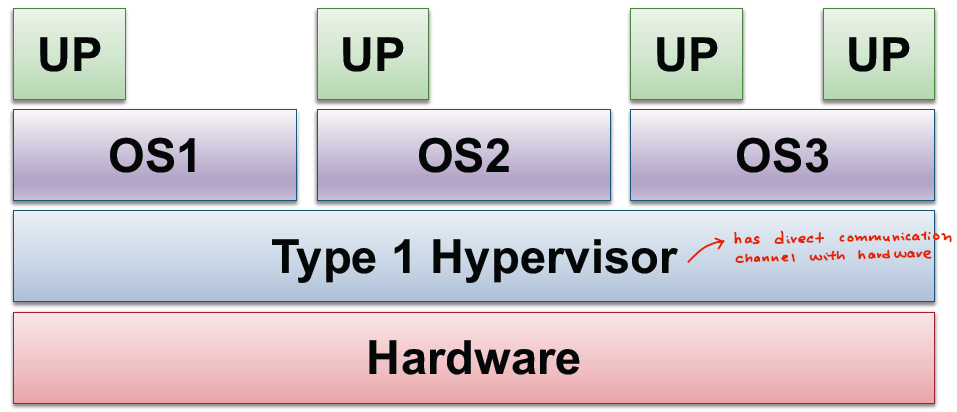
\includegraphics[width=0.39\textwidth]{type_1}%
            \qquad%
            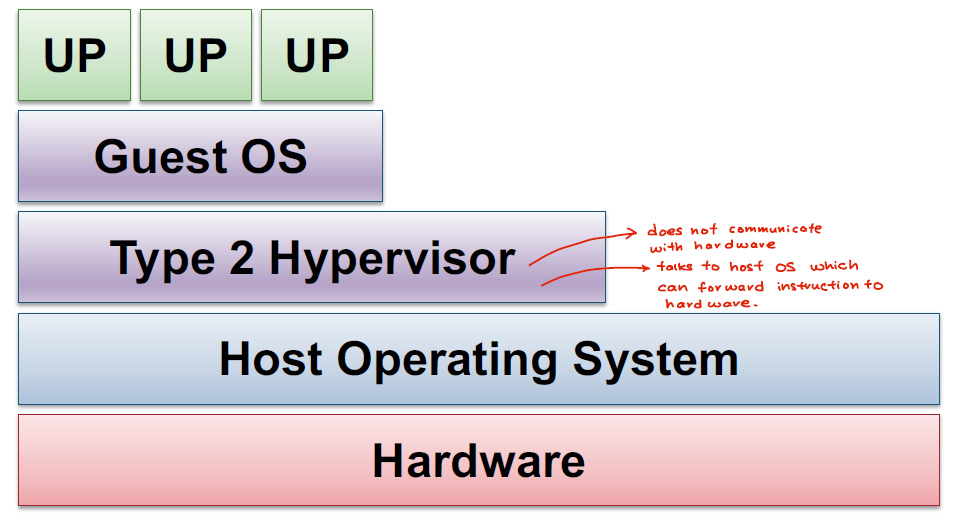
\includegraphics[width=0.39\textwidth]{type_2}%
        \end{minipage}
        \begin{center}
            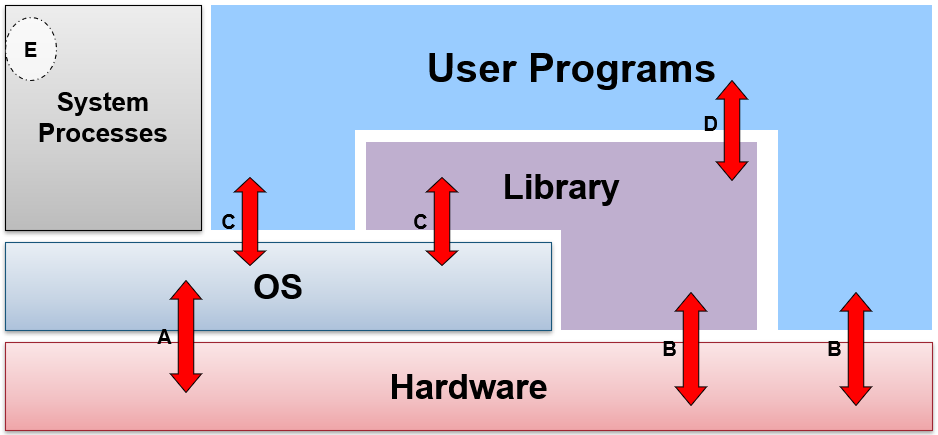
\includegraphics[width=0.35\columnwidth]{interactions}
        \end{center}
        \section{Process Abstraction}
        \subsection{Process Abstraction}
        \begin{itemize}
            \item \textbf{Process}: a dynamic abstraction for executing program
            \item Includes all information required to describe a running program (Memory context, hardware context, OS context)
            \item Information is used to \textbf{context switch} between running programs (to switch from program A to B, we save all information regarding program A then load information of program B)
            \item An executable binary consists of two major components: instructions and data
            \item During execution, more information:
            \begin{itemize}
                \item \textbf{Memory context}: text, data, stack, heap
                \item \textbf{Hardware context}: General Purpose Registers, Program Counter, Stack Pointer, Stack FP, ...
                \item \textbf{OS context}: PID, Process state, Resources used, File Descriptor
            \end{itemize}
        \end{itemize}
        \begin{tabular}{l}
            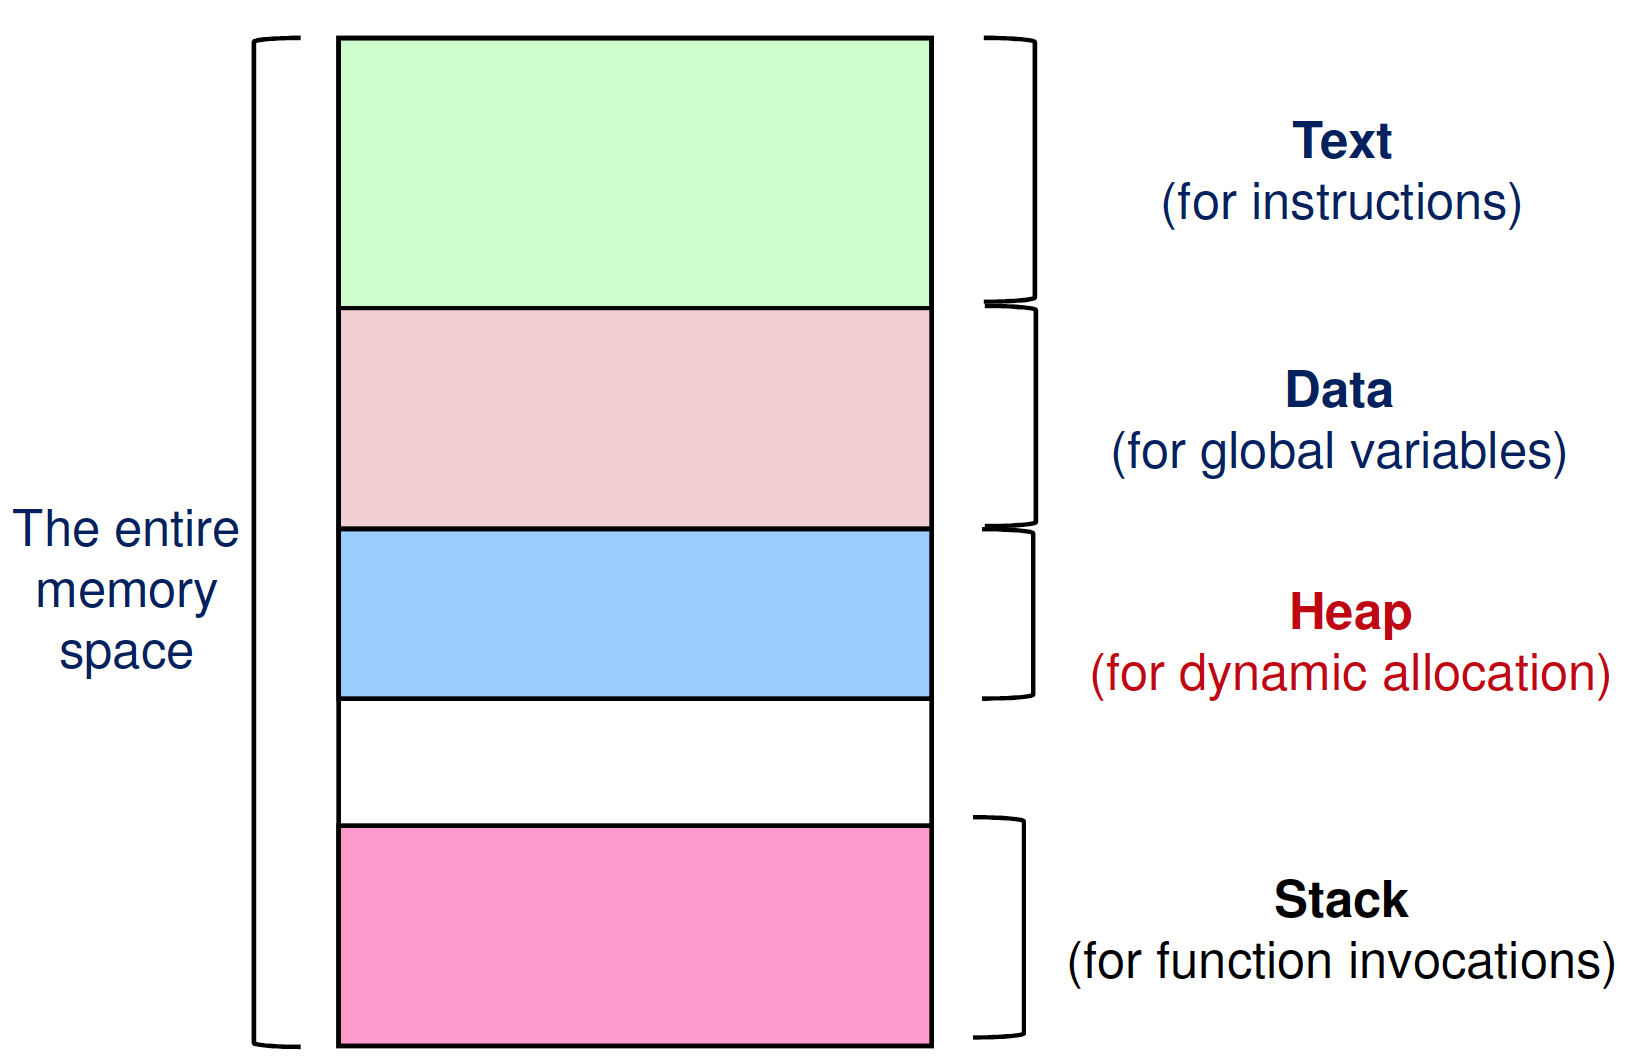
\includegraphics[width=0.5\linewidth]{stack-memory}
        \end{tabular}
        \begin{tabularx}{0.45\columnwidth}{X}
            Note: stack grow upwards in this case
        \end{tabularx}
        \subsection{Memory Hierarchy}
        \begin{center}
            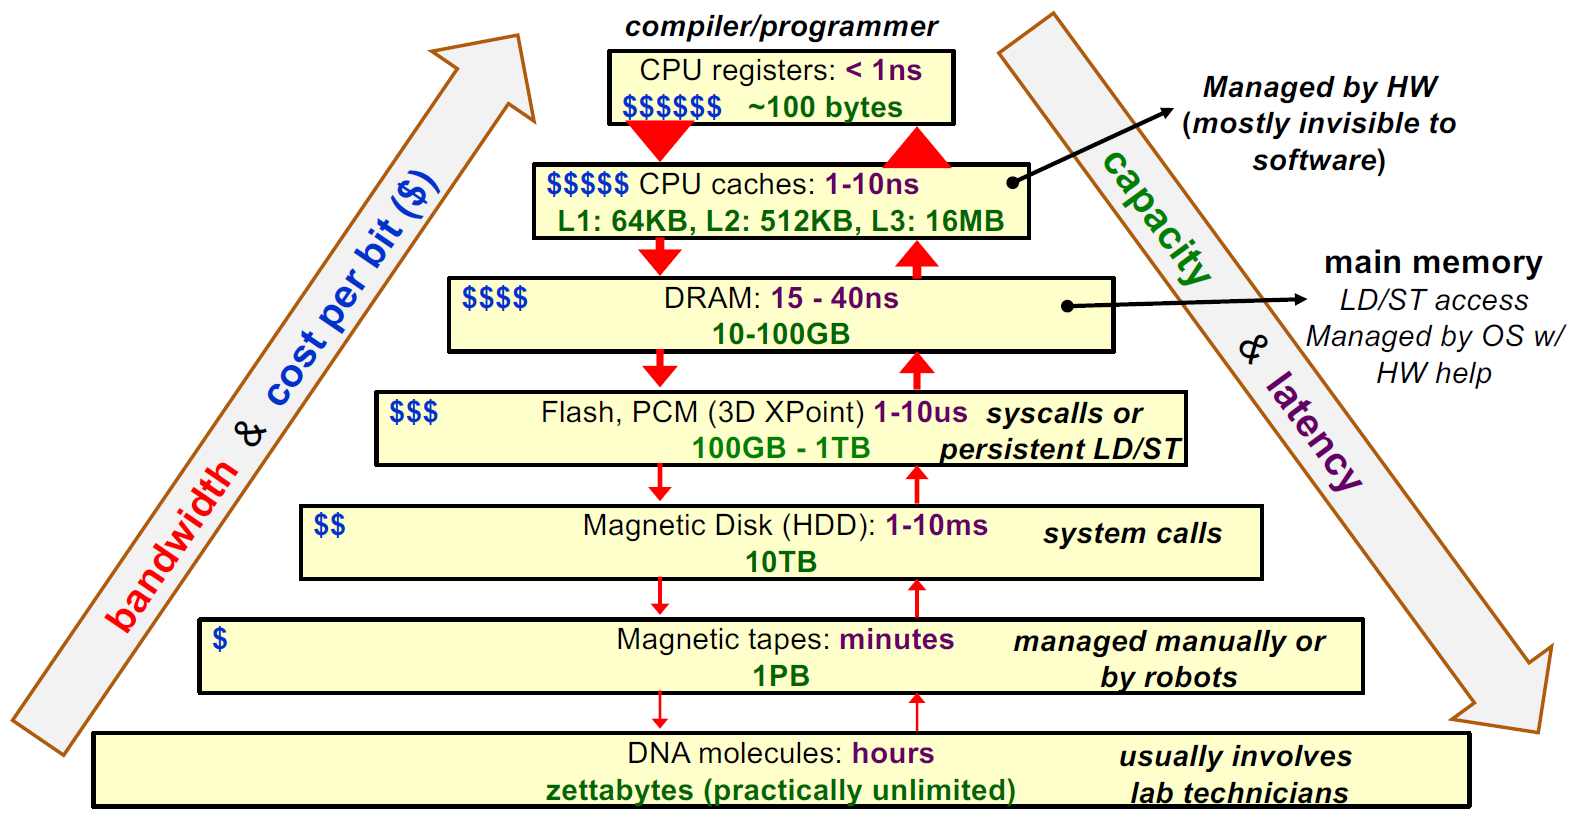
\includegraphics[scale=0.17]{memory_hierarchy}
        \end{center}
        \subsubsection{Caches}
        Caches duplicate part of the memory for faster access (hardware optimization), are fast and invisible to software, usually split into instruction and data cache (optimized differently)
        \subsection{Function calls}
        \subsubsection{Challenges faced when calling functions}
        \begin{itemize}
            \item How to differentiate between global variables and local variables?
            \item Once we return from a function where do we return to? There is no static point of return from a function.
        \end{itemize}
        \subsubsection{Control Flow and Data}
        Important steps (and their corresponding issues):
        \begin{enumerate}
            \item Setup the parameters (Setup "per-function data")
            \item Transfer control to callee (Need some way to jump to function)
            \item Setup local variables (How do we store this so there is no conflict?)
            \item Store result if applicable (Need some way to capture return result)
            \item Return to caller (How do we know where to return to?)
        \end{enumerate}
        \subsection{Stack Memory (LIFO data structure)}
        \begin{itemize}
            \item New memory region to store information of a function invocation
            \item Described by a \textbf{stack frame}, containing: Return address of the caller (PC, old SP), Arguments for the function, Storage for local variables, Frame Pointer, Saved Registers
            \item \textbf{Stack Pointer} = The top of stack region (first unused location)
            \item \textbf{Frame Pointer} = points to a \textbf{fixed location in a stack frame} (platform dependent)
            \item \textbf{Saved Registers} = memory to temporarily hold General Purpose Registers (GPR) value during \textbf{register spilling}* since number of registers are very limited
        \end{itemize}
        * Register spilling occurs when GPRs are exhausted and have to be temporarily be stored on memory so they can be reused
        \subsubsection{Function Call Convention}
        Setup and teardown of the stack frame is usually \textcolor{red}{done by the programmer or the compiler} (we usually don't want the OS to touch the stack)\\\\
        \textbf{Stack Frame Setup}:
        \begin{itemize}
            \item \textbf{Caller}: Pass parameters with registers and/or stack, Save Return PC on stack
            \item \textbf{Callee}: Save the old FP, SP, and registers used by callee, Allocate space for local vars on stack, adjust SP to point to new stack top\\
        \end{itemize}
        \textbf{Stack Frame Teardown}:
        \begin{itemize}
            \item \textbf{Callee}: Place return result on stack, Restore saved registers, FP, SP
            \item \textbf{Caller}: Utilize return result, Continues execution
        \end{itemize}
        \subsection{Dynamically Allocated Memory}
        Using a separate \textbf{heap memory region} that allows for memory space to be acquired during execution time. \textbf{Grows in opposite direction from stack}: to allow for more flexibility since there are times we need more stack memory (e.g. recursion) and sometimes we need more heap memory
        \subsubsection{Behaviour of heap}
        \begin{enumerate}
            \item Allocated only at runtime: size not known during compilation time $\rightarrow$ cannot be placed in Data region
            \item No definite deallocation timing: can be explicitly freed by programmer or implicitly freed by garbage collector $\rightarrow$ cannot be placed on stack
            \item Tends to create "holes" or "fragments" in memory since any portion of the heap can be deallocated at any time $\rightarrow$ need to run defragment programs to compact the heap
        \end{enumerate}
        \subsection{Process Identification \& Process State}
        \begin{itemize}
            \item Using process ID \textbf{(PID)}, a unique number among the processes.
            \item OS dependent issues: Are PID's reused? Are there reserved PID's? Does it limit max number of processes?
        \end{itemize}
        \begin{center}
            \textbf{5 State Process Model}:\\
            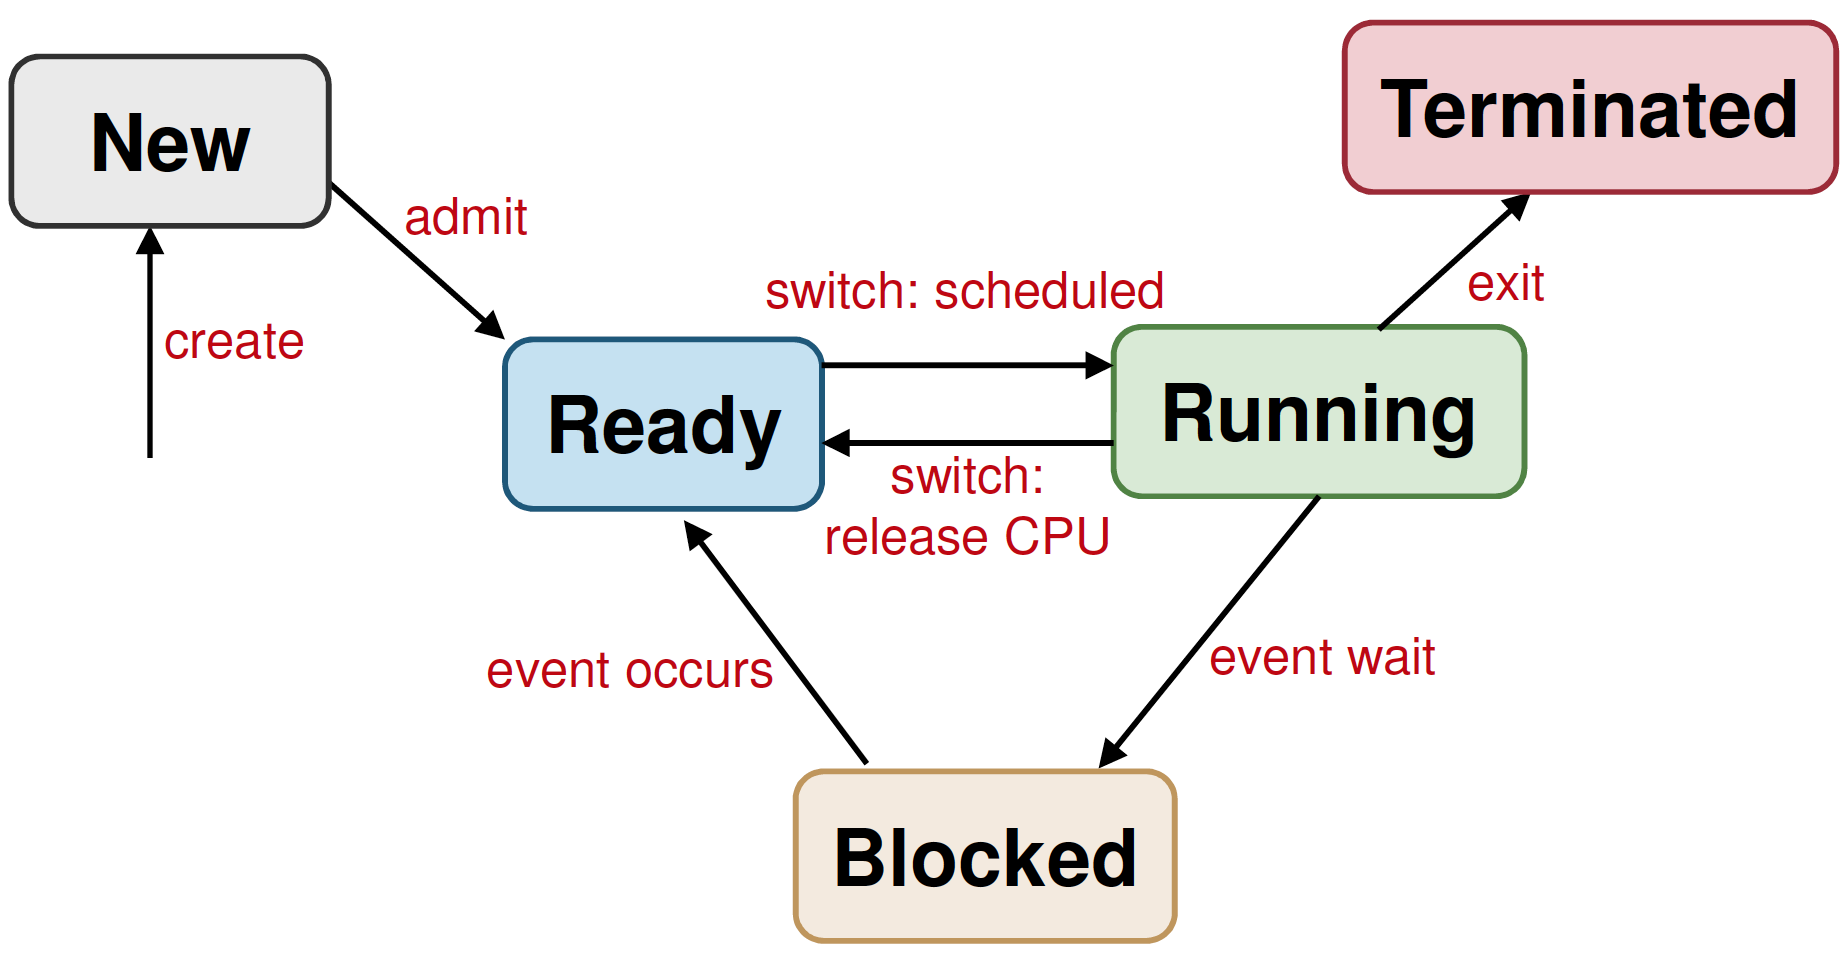
\includegraphics[width=0.7\linewidth]{process-state}
        \end{center}
        \begin{enumerate}
            \item \textbf{New}: process created, may still be initialising, not yet ready
            \item \textbf{Ready}: process is admitted by scheduler waiting to run
            \item \textbf{Running}: process being executed on CPU
            \item \textbf{Blocked}: process waiting, can't execute till event is available
            \item \textbf{Terminated}: process finished execution, may require OS cleanup
        \end{enumerate}
        \textbf{Transitions}:
        \begin{itemize}
            \item nil -> New (Create)
            \item New -> Ready (Admit): Process ready to be scheduled
            \item Ready -> Running (Switch): Process selected to run
            \item Running -> Ready (Switch): Process gives up CPU voluntarily or preempted by scheduler
            \item Running -> Blocked (Event wait): e.g. syscall, waiting for I/O, ...
            \item Blocked -> Ready (Event occurs)
        \end{itemize}
        \textbf{With 1 CPU}:
        \begin{itemize}
            \item $\leq$ 1 process in running state
            \item conceptually 1 transition at a time
        \end{itemize}
        \textbf{With m CPUs}:
        \begin{itemize}
            \item $\leq$ m processes in running state
            \item possibly parallel transitions
            \item each process may be in different states
        \end{itemize}
        \subsection{Process Table \& Process Control Block}
        \begin{tabularx}{0.42\columnwidth}{X}
            \begin{itemize}
                \item \textbf{PCB/Process Table Entry} = entire execution context for a process
                \item \textbf{Process Table} =  kernel maintains PCB for all processes, stored as one table
                \item Stores a bunch of pointers that points to the correct places so that processes can be restored after context switch
                \item Issues: Scalability, Efficiency
            \end{itemize}
        \end{tabularx}
        \begin{tabular}{l}
            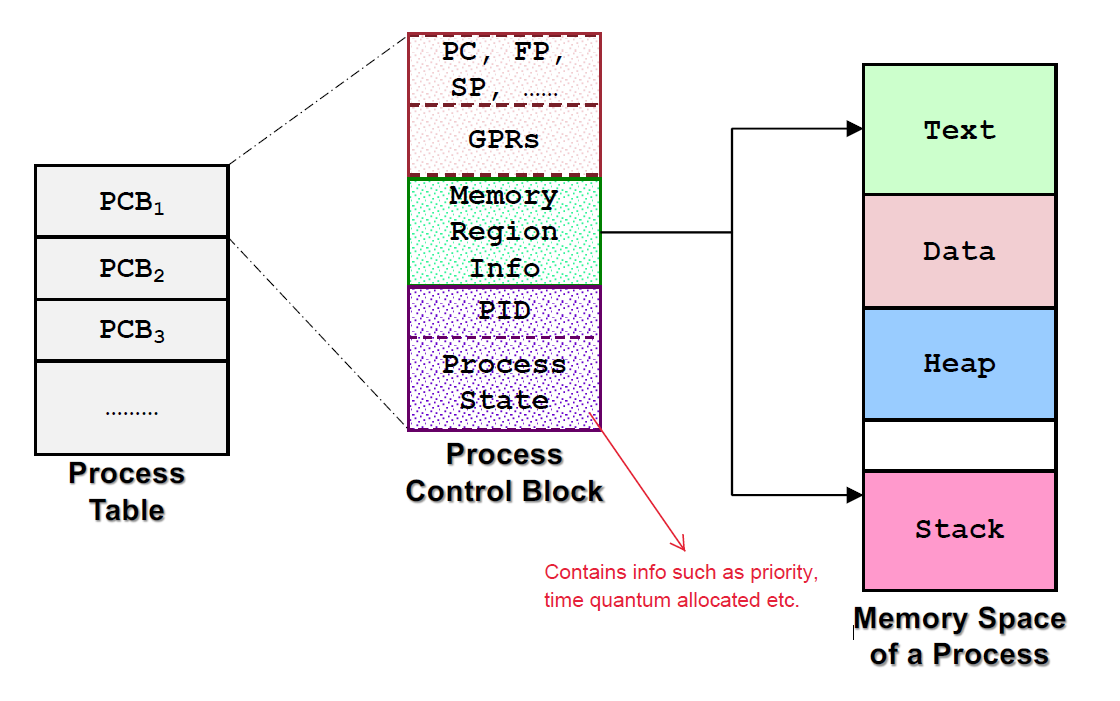
\includegraphics[width=0.55\linewidth]{process-table}
        \end{tabular}
        \subsection{System Calls}
        API to OS -- provides a way of calling services in kernel, different from normal function call in that have to change from user mode -> kernel mode, more expensive due to OS overhead
        \subsubsection{APIs in different OS}
        \begin{itemize}
            \item Unix variants mostly follows POSIX (portable operating interface) standards and typically have a small number of system calls: ~100
            \item Windows uses Win API which typically have a huge number of system calls: ~1000, and new system calls comes with each new version
        \end{itemize}
        \subsubsection{C/C++ Sys calls}
        A C/C++ program can call the library version of system calls. A function wrapper has same name and parameters as the syscall. Alternatively, there is also a function adapter which is user-friendlier (less params, more flexible params value).
        \vfill\null
        \subsubsection{Sys Call Mechanism}
        \begin{enumerate}
            \item User program invokes the library call (normal function call mechanism)
            \item Library call places the system call number in a register
            \item Library call executes \texttt{TRAP} to switch from user mode to kernel mode
            \item In kernel mode, syscall handler is determined using the syscall number as index by \textbf{dispatcher}
            \item System call handler is executed
            \item System call handler ended, control return to library call, switch kernel -> user mode
            \item Library call return to user program via normal function return mechanism
        \end{enumerate}
        * syscall handlers are ptr to functions and are stored in a table to provide efficient lookup
        \subsection{Exception \& Interrupt}
        \textbf{Exception}:
        \begin{itemize}
            \item \textbf{Synchronous}, occurring due to program execution
            \item Effect: have to execute an \textbf{exception handler}, similar to a forced function call
            \item Can explicitly call \texttt{TRAP} to purposely throw exception $\rightarrow$ typically used for debugging
            \item e.g. Overflow, underflow, Divide by 0, Illegal mem address
        \end{itemize}
        \textbf{Interrupt}:
        \begin{itemize}
            \item External events interrupting execution, usually hardware-related (timer, mouse moved, keyboard pressed)
            \item \textbf{Asynchronous}, occurring independent of program execution
            \item Effect: execution is suspended, have to execute \textbf{interrupt handler}
            \item Note that if a program is in the middle of executing an instruction, it would complete that instruction first before passing control to interrupt
            \item Interrupts can be stacked (timer interrupt can take over a mouse interrupt)
        \end{itemize}
        \subsubsection{Handler Routine}
        \begin{enumerate}
            \item Save register/CPU state
            \item Perform handler routine
            \item Restore register/CPU
            \item Return from interrupt
        \end{enumerate}
        * Exception uses software for handler routine whereas interrupts uses hardware\\
        * Handler uses a different hardware context than user programs
        \section{Process Abstraction: Unix}
        \subsection{Process in UNIX}
        Contains information on PID, Process state (running, sleeping, stopped, zombie), Parent PID (PPID), Cumulative CPU time etc.
        \subsection{Process Creation: Fork}
        Fork creates a new process known as \textbf{child process} which is a duplicate of the current executable image (same code, same address space, same PC etc.). \textcolor{red}{Data is a copy of the parent }(i.e. not shared). Only differs in PID, PPID and \texttt{fork()} return value (0 for child and > 0 for parent).
        \subsection{Common UNIX syscalls}
        \begin{itemize}
            \item \mintinline{C}{int execl(char *path, char *arg0, ..., char *argN, NULL);} replaces current executing process image, \textcolor{red}{does not return unless error}. Will not exit on error. Only replaces Code and does not replace PID and other information
            \item \mintinline{C}{void exit(int status);} \texttt{Status} is returned to parent process and has value 0 to represent normal termination, else problematic. Does not return.
            \item \mintinline{C}{int wait(int *status);} returns the PID of terminated child (\textcolor{red}{does not wait for grandchildren}), status stores exit status. Blocking (\textcolor{red}{does not block when process has no children}). Cleans up remainder of child system resources. Note that \textcolor{red}{\texttt{wait()} waits for child even if child calls \texttt{execl()}}
        \end{itemize}
        \subsection{Master Process}
        The common ancestor of all processes is \texttt{init} which is created in kernel at boot up time and has a PID = 1
        \subsection{Process Termination}
        Most system resources used by process are released on exit. Only PID, status and CPU time are not released (to facilitate clean up by parent when it calls \texttt{wait}). Generally, PCB is also not removed. On program termination, open files are flushed automatically.\\\\
        \textbf{Zombie process}: child process terminates but parent did not call \texttt{wait} -- child becomes zombie, can fill up processs table, created so that \texttt{wait()} system call can work properly, user command running in the background is considered a zombie\\
        \textbf{Orphaned Process}: parent terminates before child -- \texttt{init} becomes pseudo-parent, who will call \texttt{wait} on children
        \subsection{Implementing \texttt{\textbf{fork()}}}
        Simplified implementation:
        \begin{enumerate}
            \item Create address space of child process
            \item Allocate p' = \texttt{new PID}
            \item Create entry in Process Table
            \item Copy kernel environment of parent process (e.g. priority for process scheduling)
            \item Initialize child process context: \texttt{PID} = p', \texttt{PPID} = parent ID, \textcolor{red}{zero CPU time}
            \item Copy memory regions, program, stack, data (further optimized by using copy-on-write)
            \item Acquires shared resources (files, current working directory)
            \item Initialize hardware context (Copy registers from parent)
            \item Add child process to scheduler queue
        \end{enumerate}
        * \textbf{Copy-on-write} only duplicates a memory location when it is written to (either by parent or child). When data is read only, memory is shared between parent and child
        \section{Process Scheduling}
        3 categories of \textbf{processing environment}: (1) \textbf{Batch Processing}: no user, no interaction, no need to be responsive, high system utilization is critical, (2) \textbf{Interactive}: with active user interacting, need to be responsive, consistent in response time, (3) \textbf{Real-time Processing}: deadline to meet, usually periodic process
        \subsection{Criteria for Scheduling Algorithms}
        \begin{itemize}
            \item \textbf{Fairness}: fair share of CPU time, no starvation (prevalent in priorty based scheduling)
            \item \textbf{Balanceed}: all parts of the computing system should be utilised (shouldn't have a scenario where all processes are waiting on CPU or I/O)
        \end{itemize}
        \subsection{Types of scheduling policies}
        \begin{itemize}
            \item \textbf{Non-preemptive (cooperative)} -- a process stays scheduled until it blocks/gives up the CPU voluntarily
            \item \textbf{Preemptive}: CPU can be taken from running process at \textcolor{red}{ANY} time. A process is given a fixed time quota to run (possible to block or yield early), at the end of the time quota, the running process is suspended and another process gets picked.
        \end{itemize}
        \subsection{Scheduling a process}
        \begin{enumerate}
            \item Scheduler is triggered (OS takes over)
            \item If context switch is needed: context of current running process is saved, placed on blocked/ready queue
            \item Pick a suitable process \textbf{P} to run based on scheduling algorithm
            \item Setup the context for \textbf{P}
            \item Let process \textbf{P} run
        \end{enumerate}
        \subsection{Scheduling for Batch Processing}
        Criteria:
        \begin{itemize}
            \item \textbf{Turnaround time}: Total time taken (time when it end - time when it arrived), related to waiting time, waiting time = Turnaround time - Time spent doing work (CPU + I/O)
            \item \textbf{Throughput}: Rate of task completion
            \item \textbf{CPU Utilisation}: \% of time when CPU is working on a task, higher the better
        \end{itemize}
        \subsubsection{First-Come First-Served (FCFS)}
        \begin{itemize}
            \item Tasks are stored on a FIFO queue based on arrival time. Pick the head of queue to run until task is done OR task is blocked. Blocked task removed from queue, when it is ready again, placed at back of queue like a newly arrived task.
            \item \textbf{Guaranteed} to have no starvation: \# of tasks in front of task X in FIFO is always decreasing -> task X will get its chance eventually.
            \item Shortcoming: \textbf{Convoy Effect} -- due to non-preemptiveness, one slow process (CPU intensive) slows down the performance of the entire set of processes.
        \end{itemize}
        \subsubsection{Shortest Job First (SJF)}
        \begin{itemize}
            \item Select the task that needs the shortest amount of CPU time, thus \textbf{guarantees} smallest average waiting time (in turn decreasing average turnaround time).
            \item \textbf{Shortcomings}: Need to know total CPU time for a task in advance (have to guess if not available), \textbf{starvation is possible} (biased towards short jobs, long jobs may never run)
            \item Predicting CPU Time, common approach (\textbf{Exponential Average}):\\
            \textcolor{red}{$\text{Predicted}_{n+1} = \alpha \text{Actual}_n + (1-\alpha)\text{Predicted}_n$}, where $\alpha$ represents the significance of immediate past values, and $(1-\alpha)$ represents the significance of past history (typical $\alpha$ value is 1/2)
            \item Higher $\alpha$ cause predicted value to fluctuate closer to the last value, while lower $\alpha$ allow a predicted value that is closer to the historical value
        \end{itemize}
        \subsubsection{Shortest Remaining Time (SRT)}
        \begin{itemize}
            \item Select job with shortest remaining (or expected) time.
            \item Variation of SJF that is \textbf{preemptive} and uses remaining time.
            \item New job with shorter remaining time can preempt currently running job
            \item Provide good service for short jobs even when they arrive late
        \end{itemize}
        \subsection{Scheduling for Interactive Systems}
        \begin{itemize}
            \item
            Criteria:
            \begin{itemize}
                \item \textbf{Response time}: Time between request and response by system (time when it first start running - time when it first reach)
                \item \textbf{Predictability}: Lesser variation in response time $\rightarrow$ better predictability
            \end{itemize}
            \item \textbf{Preemptive} scheduling algorithms are used to ensure good response time, thus scheduler needs to run periodically.
            \item \textbf{Timer interrupt} = interrupt that goes off periodically based on hardware clock, OS ensures timer interrupt is not intercepted by other program/interrupt
            \item Timer interrupt handler \textbf{invokes OS scheduler}.
            \item \textbf{Interval of Timer Interrupt (ITI)} typically 1-10ms, scheduler is triggered every ITI but may not actually run
            \item \textbf{Time Quantum} = execution duration given to a process, can be constant/variable, must be multiple of ITI (commonly 5-100ms)
        \end{itemize}
        \subsubsection{Round Robin (RR)}
        \begin{itemize}
            \item Tasks stored in a FIFO queue, pick task from head of queue until time quantum elapsed OR task gives up CPU voluntarily OR task blocks
            \item Basically a \textbf{preemptive version of FCFS}
            \item \textbf{Response time guarantee}: given $n$ tasks and quantum $q$, time before a task get CPU is bounded by $(n-1)q$, note that \textcolor{red}{bounded response time $\neq$ responsive}
            \item Choice of time quantum: big = better CPU utilization, longer waiting time; small = bigger overhead (worse CPU utilization) but shorter waiting time
        \end{itemize}
        \subsubsection{Priority Scheduling}
        \begin{itemize}
            \item Assign a \textbf{priority} value to all tasks, select task with highest priority value.
            \item \textbf{Preemptive}: higher priority process can preempt running process with lower priority
            \item \textbf{Non-preemptive}: late coming high priority process has to wait for next round of scheduling
            \item \textbf{Shortcomings}: Low priority process \textbf{can starve}, worse in preemptive variant
            \item \textbf{Possible solutions}: Decrease the prioty of currently running process after every time quantum, Give each process a minimum time quantum
            \item Generally hard to guarantee/control exact amount of CPU time given to a process
            \item \textbf{Priority Inversion}: 3 processes, priorities Hi, Mi, Lo. L locks resource, M pre-empts L, A arrives and tries to lock same resource as L. Then M continues executing although H has higher priority.
        \end{itemize}
        \subsubsection{Multi-level Feedback Queue (MLFQ)}
        \begin{itemize}
            \item Designed to solve the issue of scheduling without perfect knowledge (e.g. no need to guess and estimate running time)
            \item Adaptive, minimising both response time for IO-bound and turnaround time for CPU-bound
            \item Rules:
            \begin{itemize}
                \item Priority(A) $>$ Priority(B) -> A runs (\textcolor{red}{after B time quantum is up})
                \item Priority(A) == Priority(B) -> A and B runs in RR
                \item New job -> highest priority
                \item If a job fully utilised its time slice -> priority reduced
                \item If a job gives up/blocks before it finishes the time slice -> priority retained
            \end{itemize}
            \item \textbf{Shortcomings}: (1) \textbf{Starvation} -- if there are too many interactive jobs, long-running jobs will starve, (2) gaming the scheduler by running for 99\% of time quantum, then relinquish the CPU (\textbf{hogging CPU}), (3) a program may change its behaviour CPU-bound -> interactive (\textbf{not given priority when it is needed})
            \item Possible solution:
            \begin{itemize}
                \item \textbf{Priority boost}: Periodically move all processes to highest priority. \textcolor{red}{guaranteeing no starvation }as highest priority -> RR, also allows processes with different behaviour phases to be treated correctly even after it reach lowest priority
                \item \textbf{Cumulative Time Quantum}: Once a job uses up its time allotment at a given level, its priority is reduced
            \end{itemize}
        \end{itemize}
        \subsubsection{Lottery Scheduling}
        \begin{itemize}
            \item Give out "lottery tickets" to processes. When a scheduling decision is needed, a ticket is chosen randomly among eligible tickets.
            \item In the long run, a process holding X\% of tickets can win X\% of the lottery held and use the resource X\% of the time.
            \item \textbf{Responsive}: newly created process can participate in next lottery, every process gets to run in every round (\textcolor{red}{waiting time is bounded by $2\times{N}\times{}$TQ})
            \item \textbf{Good level of control}: A process can be given lottery tickets to be distributed to its child process, an important process can be given more lottery tickets, each resource can have its own set of tickets
            \item Simple implementation
        \end{itemize}

        \section{Inter-Process Communication}
        \begin{itemize}
            \item 2 common IPC mechanisms: \textbf{Shared-Memory} \& \textbf{Message Passing}
            \item 2 Unix-specific IPC mechanisms: \textbf{Pipe} and \textbf{Signal}
        \end{itemize}
        \subsection{Shared-Memory}
        \begin{itemize}
            \item \textcolor{red}{Implicit communication} through reads/writes to shared variables
            \item General idea: Process $p_1$ creates a shared memory region $M$ in \textbf{\textcolor{red}{user space}}, process $p_2$ attaches $m$ to its own memory space. $p_1$ and $p_2$ can now communicate using memory region $M$. Values written to $M$ is visible to all processes that share $M$.
            \item Shared memory region is identified by a number, memory address is only generated when a process attaches to the identified region
            \item Shared memory region can be accessed by any process (set permission bits to \texttt{0666})
            \item OS involved only in creating and attaching shared memory region
            \item \textbf{Advantages}: Efficient (only initial steps involves OS), Ease of use (information of any type or size can be written easily)
            \item \textbf{Disadvantages}: Synchronisation (shared resource -> need to synchronise access), Implementation is usually harder, Limited to a single machine (software abstractions can be supported in distributed systems but less efficient)
            \item In Unix: (1) create/locate shared memory region $M$, (2) Attach $M$ to process memory space, (3) Read/Write $M$, (4) Detach $M$ from memory space after use, (5) Destroy $M$ (only 1 process does this, can only destroy if $M$ is not attached)
        \end{itemize}
        \subsection{Message Passing}
        \begin{itemize}
            \item \textcolor{red}{Explicit communication} through exchange of messages
            \item General idea: process $p_1$ prepares a message $M$ and send it to process $p_2$, $p_2$ receives the message $M$. Sending and receiving messages are generally provided using syscalls (OS mediates it $\rightarrow$ easier to implement, safer but slower since involves OS overhead)
            \item Message has to be stored in \textbf{\textcolor{red}{kernel memory space}}, every send/receive operation is a syscall
            \item \textbf{Advantages}: Portable (can be easily implemented on different processing environment), Easier synchronisation (using synchronous primitive)
            \item \textbf{Disadvantages}: Inefficient (usually requiring OS intervention), Harder to use (message usually limited in size and/or format)
        \end{itemize}
        \subsubsection{Naming \textmd{(how to identify the other party in the comm):}}
        \begin{itemize}
            \item \textbf{Direct Communication}
            \begin{itemize}
                \item Sender/receiver \textbf{explicitly} name the other party (using PID)
                \item Characteristics: 1 link/pair of communicating processes, need to know the identity of the other party
            \end{itemize}
            \item \textbf{Indirect Communication}
            \begin{itemize}
                \item Message are sent to/received (\textcolor{red}{copied}) from message storage (aka mailbox or port)
                \item Characteristic: 1 mailbox can be shared among a number of processes
                \begin{itemize}
                    \item Introduces a problem of who receives the message? There are many variations used: one-to-one, one-to-many, many-to-many, many-to-one
                    \item Since mailbox is in kernel space, OS takes care of synchronisation of message reading and writing
                \end{itemize}
            \end{itemize}
        \end{itemize}
        \begin{center}
            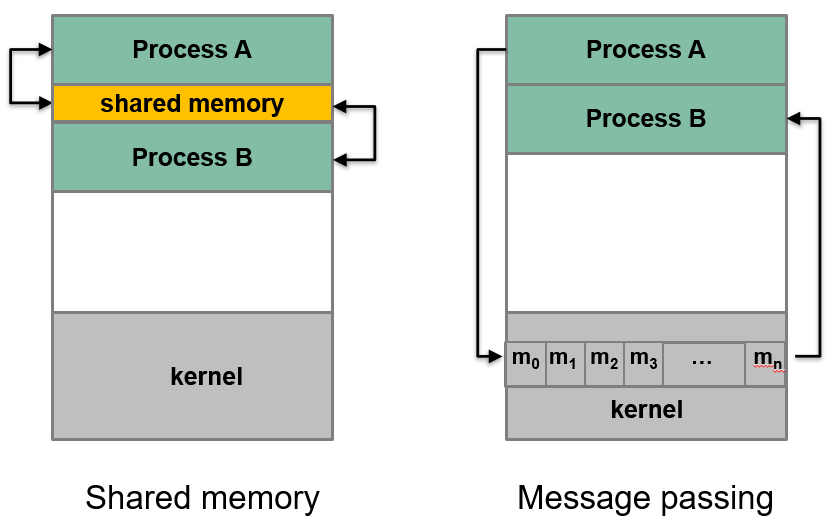
\includegraphics[width=0.57\columnwidth]{shared_vs_passing}
        \end{center}
        \subsubsection{Synchronisation \textmd{(behaviour of the sending/receiving ops)}}
        \begin{itemize}
            \item \textbf{Blocking primitives} (synchronous): sender/receiver is blocked until message is received/has arrived
            \item \textbf{Non-blocking Primitive} (asynchronous): sender resume operation immediately, receiver either receive message if available or proceeds empty handed but doesn't block
            \item Typically \texttt{receive()} is blocking $\rightarrow$ we look at the behaviour of sender to determine whether asynchronous or synchronous
        \end{itemize}
        \subsubsection{Asynchronous Message Passing}
        \begin{itemize}
            \item Assumes that \texttt{receive()} is blocking and sender is non-blocking
            \item System buffers the message (Async message passing \textbf{MUST} have a buffer)
            \item Drawbacks:
            \begin{itemize}
                \item Too much freedom for programmer, program becomes complex
                \item Finite buffer size means system is not truly asynchronous $\rightarrow$ \textcolor{red}{sender waits when buffer is full}
            \end{itemize}
            \item Buffer: Under OS control $\rightarrow$ Synchronization burden placed on OS; Decouples sender and receiver $\rightarrow$  less sensitive to variations in execution $\rightarrow$ don't have to wait on each other unnecessarily.
        \end{itemize}
        \subsubsection{Synchronous Message Passing}
        \begin{itemize}
            \item Assumes sender is blocking and receiver is also blocking
            \item \textbf{No intermediate buffers needed}
            \item \textbf{Pros}:
            \begin{itemize}
                \item Applicable \textbf{beyond single machine}
                \item \textbf{Portable}: Easily implemented on many platforms; Parties on different platforms can communicate
                \item \textbf{Easier synchronization}: Implicit, defined by blocking semantics; No shared memory region (message is copied); Achieves both communication and synchronization simultaneously
            \end{itemize}
            \item \textbf{Cons}:
            \begin{itemize}
                \item \textbf{Inefficient}: Requires OS intervention on every send/receive
                \item \textbf{Harder to use}: Requires packing/unpacking data into supported format
            \end{itemize}
        \end{itemize}
        \subsection{Unix Pipes}
        \begin{itemize}
            \item A communication channel with 2 ends, for reading and writing.
            \item A pipe can be shared between 2 processes (producer-consumer)
            \item Behaviour: like an anonymous file, \textbf{FIFO} (in-order access)
            \item Pipe functions as \textbf{circular bounded byte buffer with implicit synchronisation}: writers wait when buffer full, readers wait when buffer empty (\textbf{Async} sending)
            \item Variants: Multiple readers/writers, half-duplex (unidirectional) or full-duplex (bidirectional)
            \item \mintinline{C}{int pipe(int fd[]);} returns 0 = success. \mintinline{C}{fd[0]} reading end, \mintinline{C}{fd[1]} writing end
        \end{itemize}
        \subsection{Unix Signal}
        \begin{itemize}
            \item An \textbf{async} notification regarding an event sent to a process/thread (OS $\rightarrow$ user program OR user program $\rightarrow$ user program)
            \item Recipient of signal handle by a default set of handlers OR user-supplied handler (only applicable to some signals)
            \item Common signals in Unix: SIGKILL, SIGSTOP, SIGCONT, etc.
        \end{itemize}
        \section{Process Alternative -- Threads}
        \begin{itemize}
            \item Motivation:
            \begin{itemize}
                \item Process is expensive: under \texttt{fork()} model -- duplicate memory space and process context, context switch requires saving/restoration of process information
                \item Hard for independent processes to communicate with each other: independent memory space -- no easy way to pass information, requires Inter-Process Communication (IPC)
            \end{itemize}
            \item A \textbf{traditional process has a single thread of control} -- only one instruction of the whole program is executing at any one time. Instead, we add more threads of control such that multiple parts of the program are executing simultaneously conceptually.
            \item Essential with multi-core architectures
            \begin{itemize}
                \item \textbf{Data parallelism}: different threads doing same task on different data (typically GPU does this)
                \item \textbf{Task parallelism}: different threads do different tasks on same/different data
            \end{itemize}
        \end{itemize}
        \subsection{Process and Thread}
        \begin{itemize}
            \item A single process can have multiple threads
            \item Threads in the same process shares:
            \begin{itemize}
                \item \textbf{Memory Context}: Text, data, heap
                \item \textbf{OS Context} (PID, other resources like files, etc.)
            \end{itemize}
            \item Threads have unique:
            \begin{itemize}
                \item Identification (Thread id)
                \item Registers (general purpose \& special, including PC)
                \item Stack
            \end{itemize}
        \end{itemize}
        \subsubsection{Context Switching}
        \begin{itemize}
            \item \textbf{Process} context switch involves: OS Context, Hardware Context, Memory Context
            \item \textbf{Thread} switch within the same process involves: Hardware context (registers, "stack" -- actually just changing FP and SP)
            \item Can think of threads as a lighter weight process
        \end{itemize}
        \begin{center}
            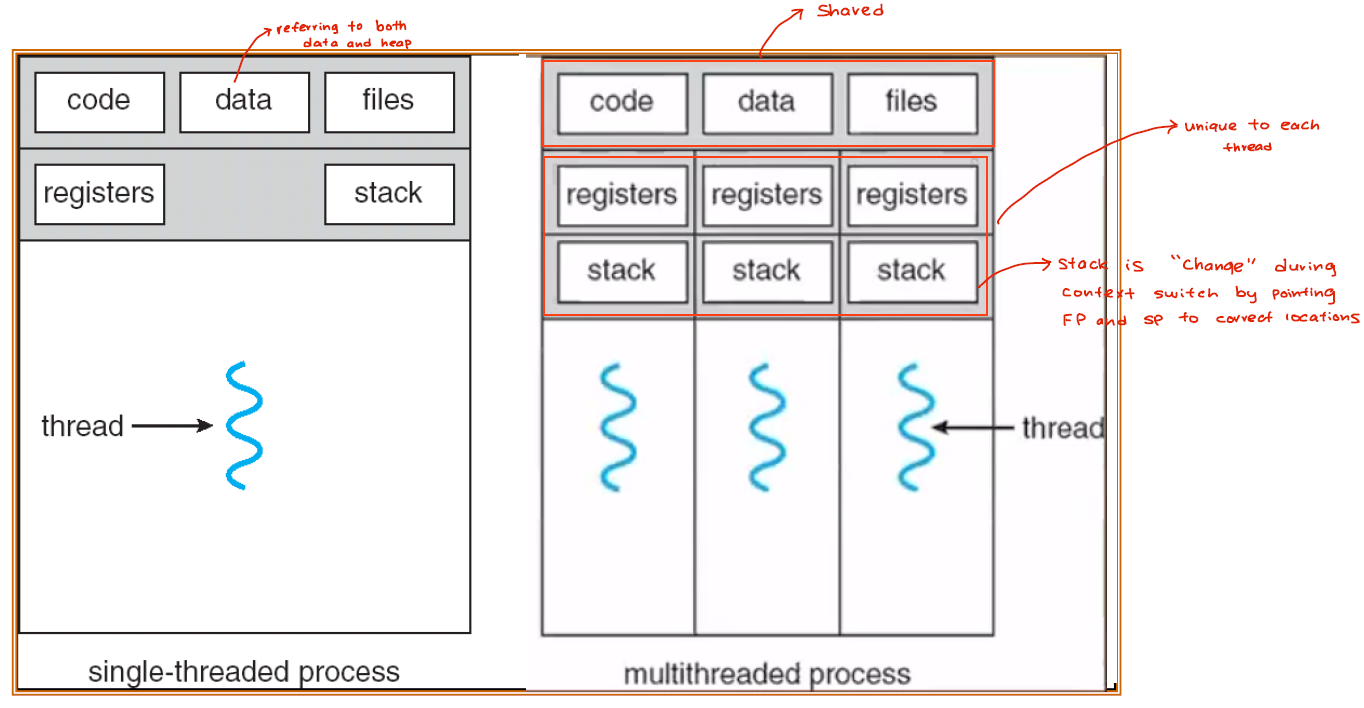
\includegraphics[width=0.65\columnwidth]{thread_illustration}
        \end{center}
        \subsection{Benefits}
        \begin{itemize}
            \item \textbf{Economy}: requires much less resources
            \item \textbf{Resource sharing}: Threads shares most resources, no need for additional information passing mechanism
            \item \textbf{Responsiveness}: multithreaded programs can appear much more responsive (one thread can deal with I/O while another is processing data)
            \item \textbf{Scalability}: Multithreaded program can take advantage of multiple CPUs
        \end{itemize}
        * Note that using threads on a SINGLE CORE does not actually speed up execution time and might instead make it run slower due to overhead
        \subsection{Problems}
        \begin{itemize}
            \item \textbf{Synchronization around shared memory is difficult to handle} -- All memory shared except the stack
            \item \textbf{System call concurrency} -- have to guarantee correctness and determine the correct behaviour of threads ran in parallel
            \item \textbf{Process behaviour} -- impact on process operations, e.g. does \texttt{fork()} duplicate threads? If single thread executes \texttt{exit()}, how abut the whole process? If a single thread calls \texttt{exec()}, how about other threads etc.
        \end{itemize}
        \subsection{Thread Models}
        \begin{itemize}
            \item \textbf{User Thread}
            \begin{itemize}
                \item Implemented as a \textbf{user library}, a runtime system in the process handles thread operations (user or library has to handle multiplexing of threads)
                \item Kernel is \textcolor{red}{not aware} of threads in the process.
                \item \textbf{Advantages}: Multithreaded program on ANY OS (ensures portability and backward compatibility), thread operations are just library calls, more configurable and flexible (such as customised thread scheduling policy)
                \item \textbf{Disadvantages}: OS is not aware of threads, scheduling is performed at \textcolor{red}{process level}. One thread blocked $\rightarrow$ process blocked $\rightarrow$ all threads blocked, cannot exploit multiple CPUs (1 solution is to do Async I/O operation)
            \end{itemize}
            \begin{center}
                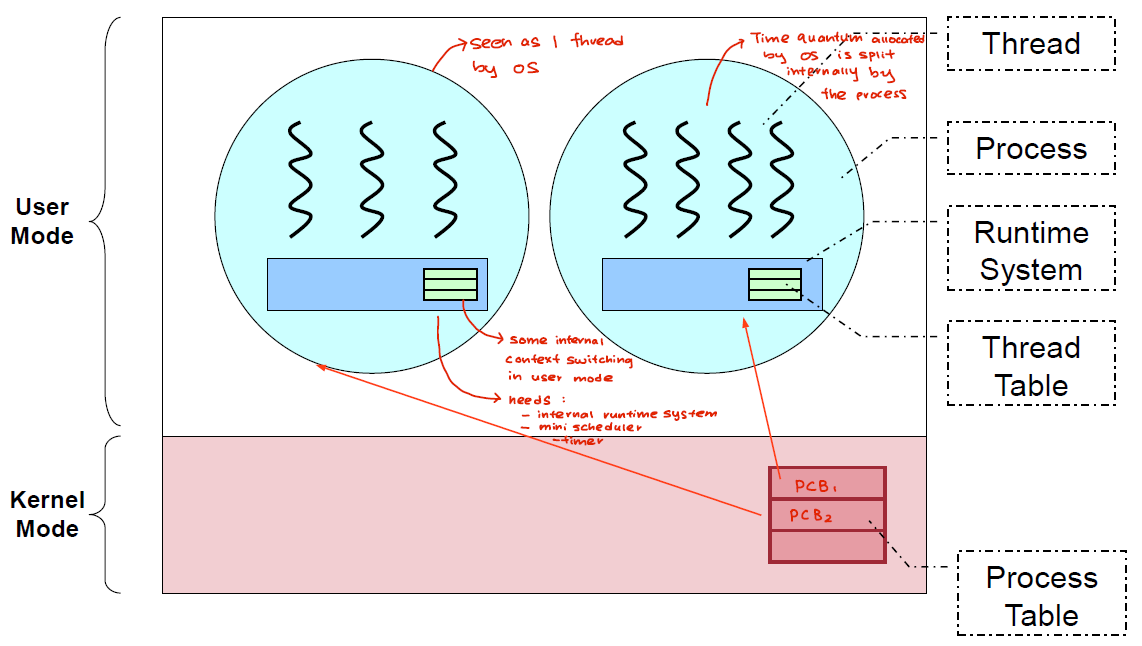
\includegraphics[width=0.65\columnwidth]{user_thread}
            \end{center}
            \item \textbf{Kernel Thread}
            \begin{itemize}
                \item Implemented in the \textbf{OS}, thread operation handled as \textbf{system calls}.
                \item Allows for \textcolor{red}{Thread-level scheduling}, basically treat kernel threads as its own process
                \item Kernel may make use of threads for its own execution
                \item \textbf{Advantages}: Kernel can schedule on thread level (threads on same process can run simultaneously on multiple CPUs $\rightarrow$ 1 thread can be blocked and the rest can still run)
                \item \textbf{Disadvantages}: Thread operation is a syscall (slower and more resource intensive), generally less flexible (used by all multithreaded programs -- many features: expensive, overkill for simple program, few features: not flexible enough for some)
            \end{itemize}
            \begin{center}
                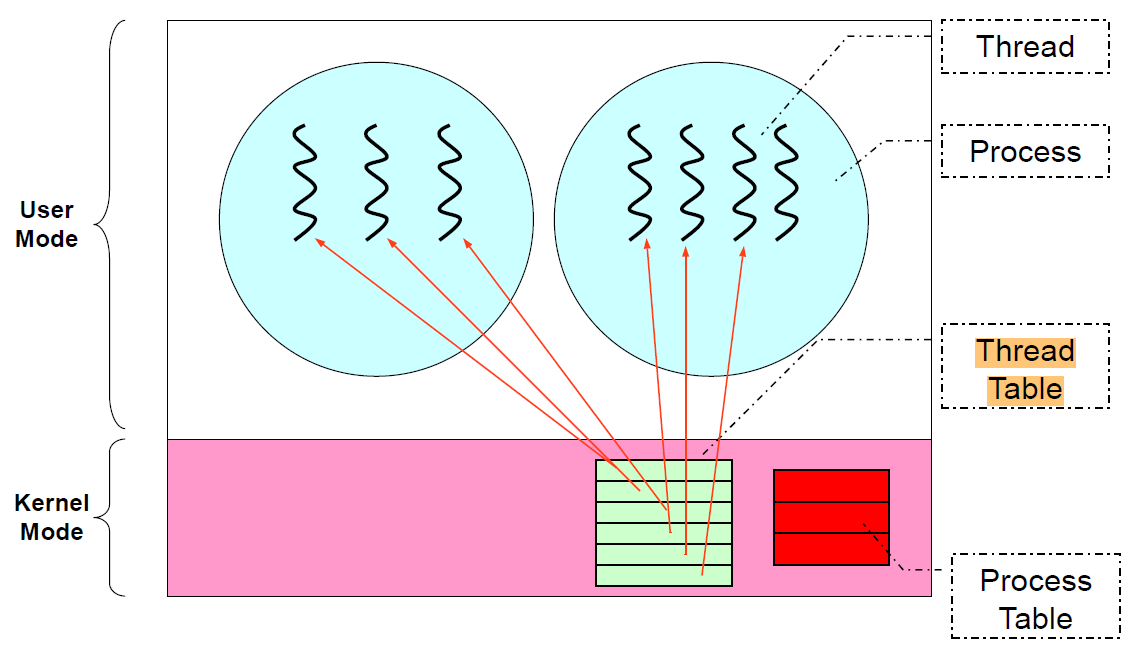
\includegraphics[width=0.65\columnwidth]{kernel_thread}
            \end{center}
            \item \textbf{Hybrid Thread Model}:
            \begin{itemize}
                \item Have \textbf{both kernel and user threads}, OS schedule on kernel threads only, user thread can bind to a kernel thread.
                \item Great flexibility (can limit concurrency of any process/user)
            \end{itemize}
            \begin{center}
                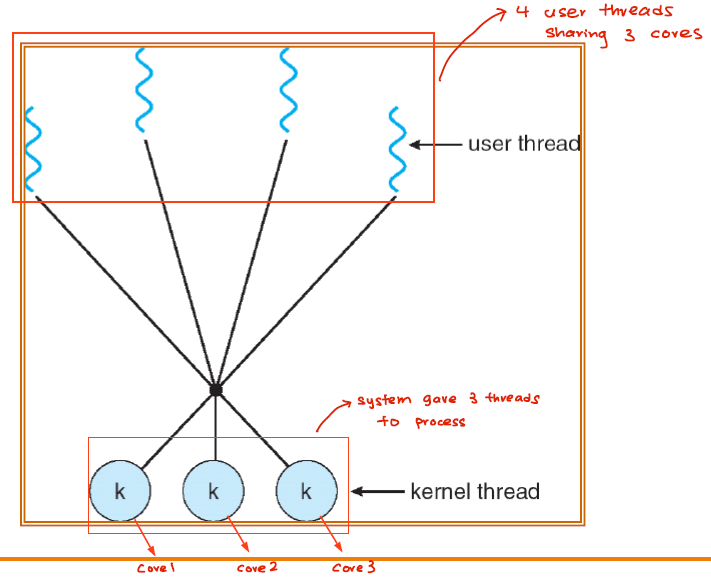
\includegraphics[width=0.7\columnwidth]{hybrid_thread}
            \end{center}
        \end{itemize}
        \subsection{Threads on Modern Processor (Intel Hyperthreading)}
        \begin{itemize}
            \item Threads started off as software mechanism: Userspace lib -> OS aware mechanism
            \item Hardware support on modern processors, supplying multiple sets of registers to \textbf{allow threads to run natively and parallelly on the same core}: \textcolor{red}{Simultaneous Multi-Threading (SMT)}
        \end{itemize}
        \subsection{POSIX Threads: \texttt{pthread}}
        \begin{itemize}
            \item Standard by IEEE, defining API and behaviour.
            \item Implementation is not specified $\rightarrow$ pthread can be implemented as user thread (windows) or kernel thread (Linux)
            \item \mintinline{C}{int pthread_create(pthread_t* tidCreated, const pthread_attr_t* threadAttributes, void* (*startRoutine) (void*), void* argForStartRoutine);}
            \begin{itemize}
                \item \texttt{tidCreated}: Thread ID for the created thread
                \item \texttt{threadAttributes}: Control the behaviour of new thread
                \item \texttt{startRoutine}: Function pointer to the function to be executed by thread
                \item \texttt{argForStartRoutine}: Arguments for the startRoutine function
            \end{itemize}
            \item \mintinline{C}|int pthread_exit(void* exitValue)|
            \begin{itemize}
                \item if \texttt{pthread\_exit()} is not called, a pthread will terminate automatically at the end of startRoutine
                \item if \texttt{"return XYZ"} is used, the "XYZ" is captured as exit value
            \end{itemize}
            \item \mintinline{C}{int pthread_join(pthread_t threadID, void **status);}
            \begin{itemize}
                \item threadID: \texttt{TID} of the pthread to wait for
                \item status: Exit value returned by the pthread
            \end{itemize}
            \item except for \texttt{pthread\_exit}, return 0 = success
        \end{itemize}
        \vfill\null
        \columnbreak
        \section{Synchronization}
        \subsection{Race Condition}
        \begin{itemize}
            \item When 2/more processes \textbf{execute concurrently} in interleaving fashion AND \textbf{share a modifiable resource} resulting in non-deterministic execution.
            \item \textbf{Solution}: designate code segment with race condition as \textbf{critical section} where at any point in time only 1 process can execute. Ideally, process in critical section should be done atomically (you either do it or you don't, cannot be done "halfway")
        \end{itemize}
        \subsection{Critical Section}
        Properties of correct implementation:
        \begin{itemize}
            \item \textbf{Mutual Exclusion}: if a process is executing in critical section, all other processes are prevented from entering it (\textbf{most critical property}, if this fails we disregard the rest)
            \item \textbf{Progress}: If no process is in critical section, one of the waiting processes should be granted access
            \item \textbf{Bounded Wait}: After a process $p_i$ requests to enter the critical section, $\exists$ an upper-bound of number of times other processes can enter the critical section before $p_i$
            \item \textbf{Independence}: process not executing in critical section should never block other processes
        \end{itemize}
        * Note that \textbf{Progress and Independence are related}. Not possible to have progress but no independence but possible to have independence but no progress (Attempt 3)
        \subsubsection{Symptoms of incorrect synchronisation}
        \begin{itemize}
            \item usually due to lack of mutual exclusion
            \item \textbf{Deadlock}: all processes \textcolor{red}{blocked} $\rightarrow$ no progress (e.g. 2 processes using message passing, both processes are using blocking receive and waiting to receive msg from the other). Fulfils the following conditions:
            \begin{enumerate}
                \item \textbf{Mutual Exlusion}: Each resource is either assigned to exactly one process or to none
                \item \textbf{Hold-and-wait}: Processes holding resources can ask for more resources
                \item \textbf{No-preemption}: Cannot forcibly take away resources previously given
                \item \textbf{Circular wait}: Must have a circular list of two or more processes, each waiting for a resource held by the next
            \end{enumerate}
            \item \textbf{Livelock}: processes keep changing state to avoid deadlock and make no other progress, typically \textcolor{red}{processes are not blocked}
            \item \textbf{Starvation}: some processes are blocked forever
        \end{itemize}
        \subsection{Implementations of Critical Section}
        \subsubsection{Incorrect Attempt 1}
        \begin{center}
            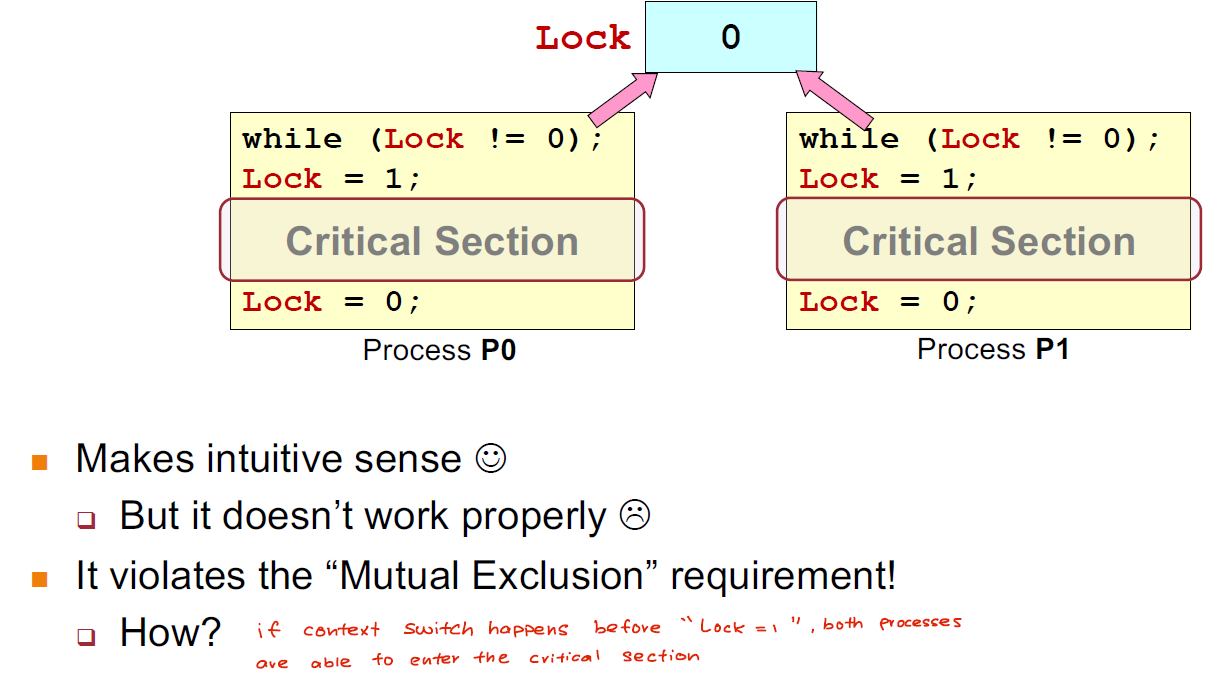
\includegraphics[width=0.9\columnwidth]{attempt1}
        \end{center}
        \subsubsection{Attempt 1 Incorrect Fix}
        \begin{center}
            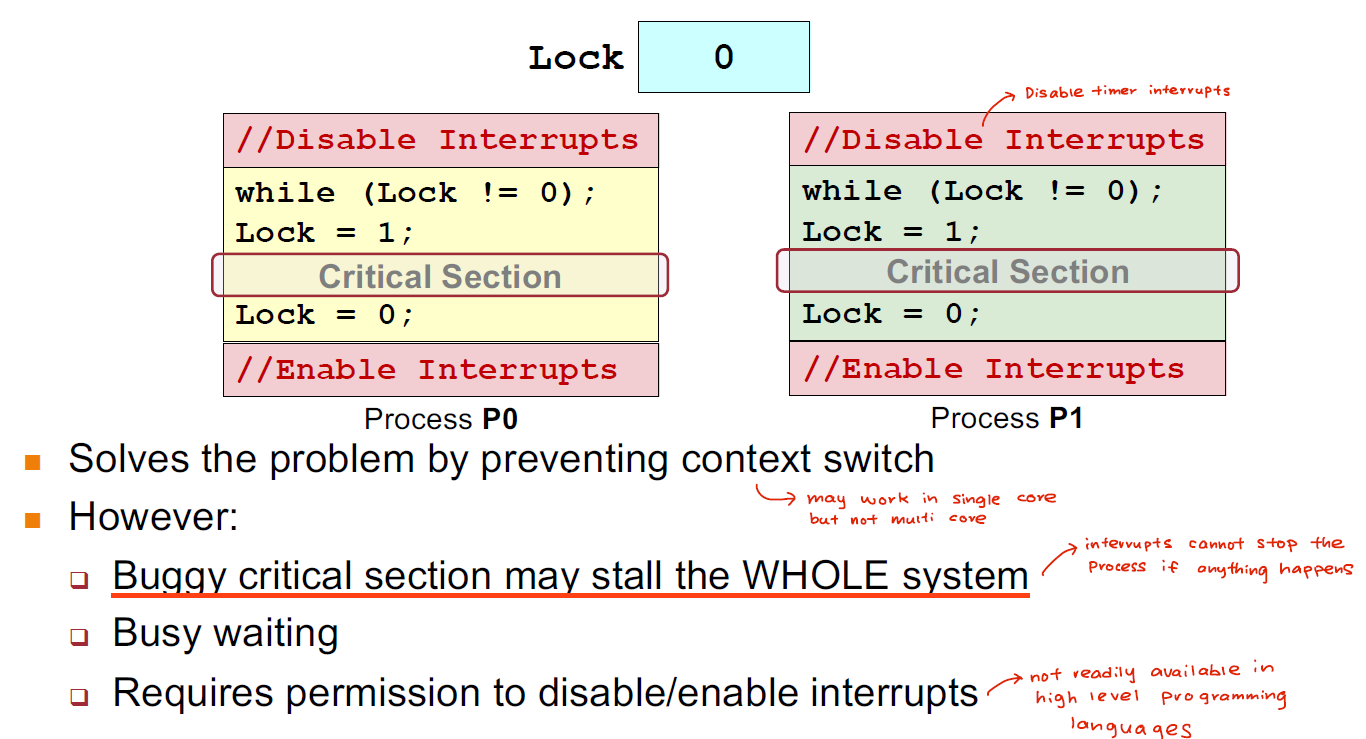
\includegraphics[width=0.9\columnwidth]{attempt_1_fix}
        \end{center}
        \subsubsection{Incorrect Attempt 2}
        \begin{center}
            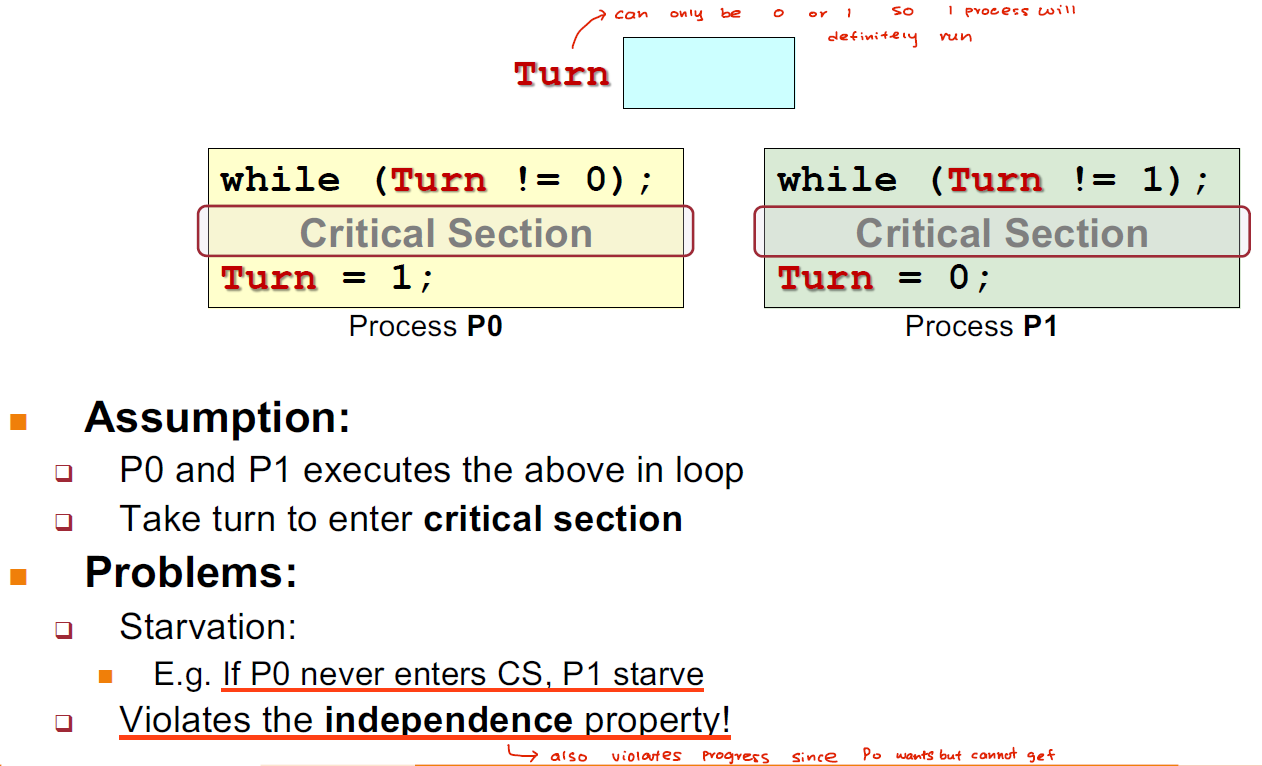
\includegraphics[width=0.9\columnwidth]{attempt2}
        \end{center}
        \subsubsection{Incorrect Attempt 3}
        \begin{center}
            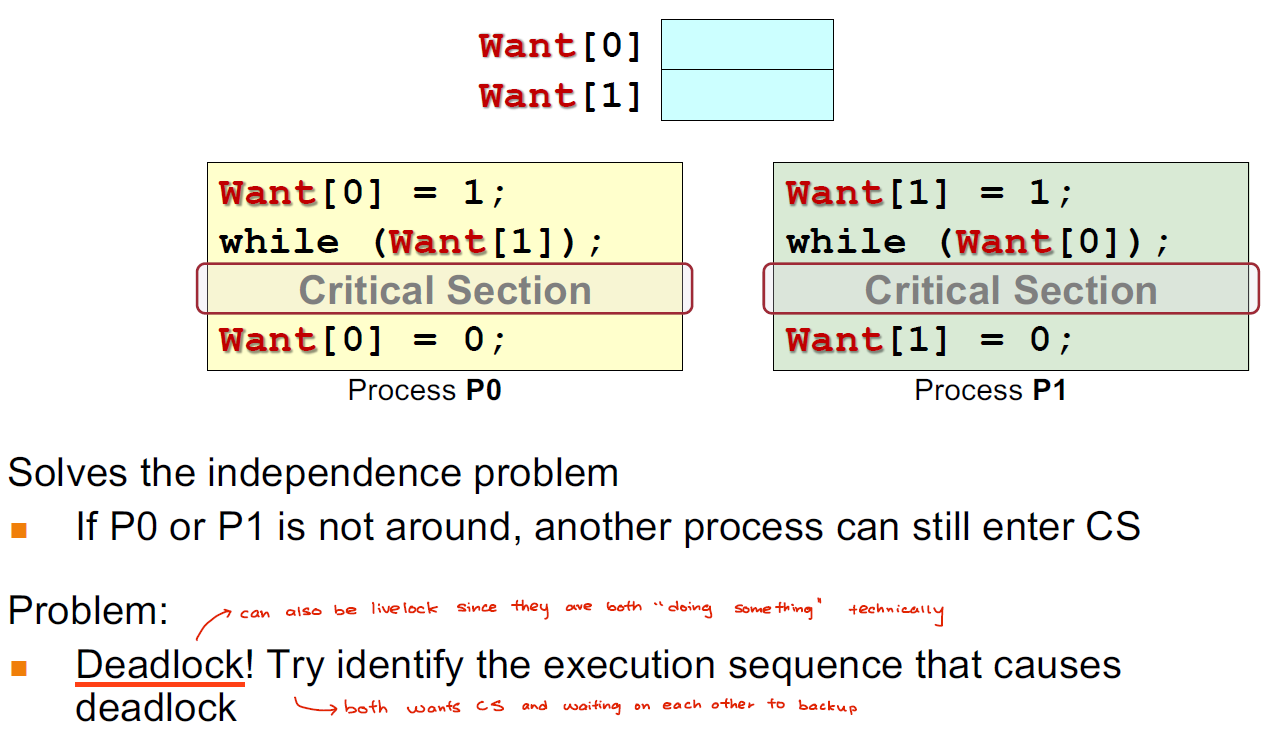
\includegraphics[width=0.9\columnwidth]{attempt3}
        \end{center}
        \subsubsection{Peterson's Algorithms}
        \begin{center}
            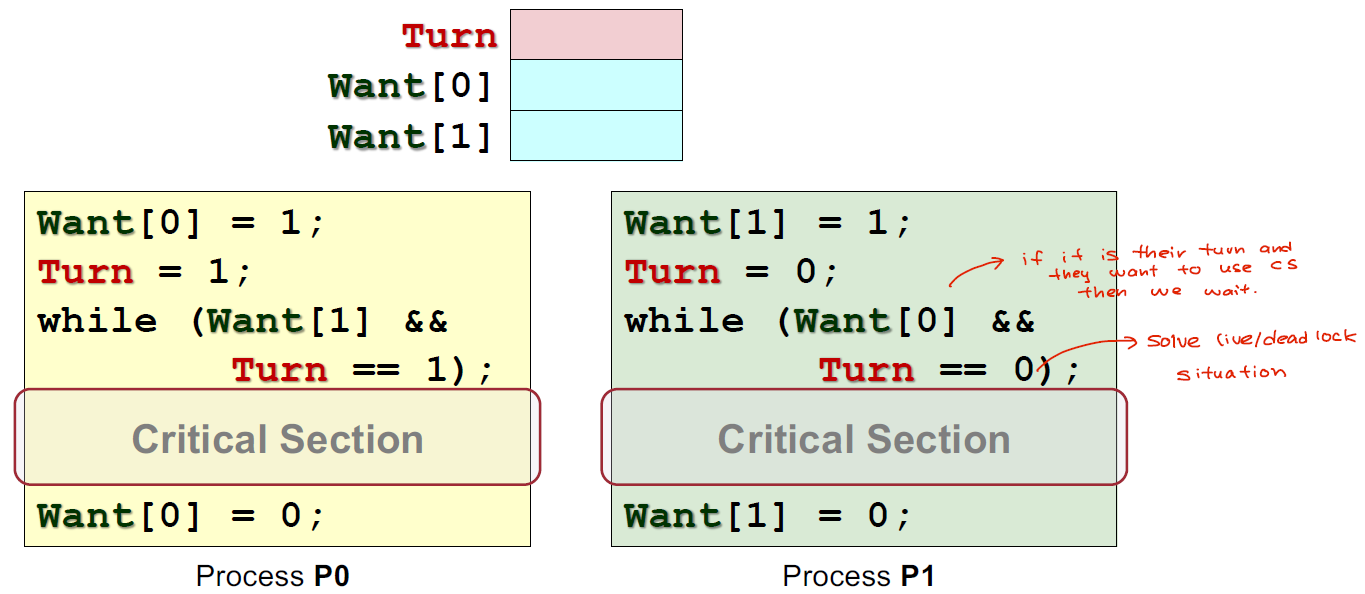
\includegraphics[width=0.9\columnwidth]{peterson}
        \end{center}
        * Note that the order of \texttt{Want[X] = 1} followed by \texttt{Turn = X} is important!
        \subsubsection{Peterson's Algorithm Disadvantages}
        \begin{itemize}
            \item \textbf{Busy Waiting}: wasteful use of processing power due to having while-loop instead of going into blocked state
            \item \textbf{Low level}: higher-level programming construct desirable to simplify mutex, make it less error prone and simpler to implement
            \item \textbf{Not general}: general synchronisation mechanism is desirable, not just mutex (limited to 2 processes)
        \end{itemize}
        \subsubsection{Test-and-set: an atomic instruction}
        \begin{itemize}
            \item Uses machine instructions to aid synchronization.
            \item Syntax: \texttt{TestAndSet Register, MemoryLocation}
            \item Load the current content at \texttt{MemoryLocation} into \texttt{Register}, Stores a \texttt{1} into \texttt{MemoryLocation}
            \item TestAndSet is performed as a single \textcolor{red}{atomic} machine operation and is \textbf{atomic even in multi-core system}
            \item Disadvantage: busy waiting (spin lock) -- wasteful use of processing power; Does not guarantee bounded-wait (unless scheduling is fair)
        \end{itemize}
        \subsubsection{Semaphore}
        A generalised synchronisation mechanism, providing a way to block a number of processes and a way to unblock one/more sleeping process(es)
        \begin{itemize}
            \item \texttt{wait(S)}: if $S > 0$, decrement. If $S \leq 0$, go to sleep
            \item \texttt{signal(S)}: increment $S$, wakes up one sleeping process (usually the first process that was blocked on semaphore (FIFO)) (if any), operation \textcolor{red}{never blocks}
            \item done with the help of OS to ensure atomicity
            \item \textcolor{red}{no busy waiting} (processes are blocked while waiting)
            \item solves all known synchronization problems
        \end{itemize}
        \textbf{Properties}
        \begin{itemize}
            \item Given $S_\text{initial} \geq 0$, where \#signal(S) = number of \texttt{signal()} executed, \#wait(S) = number of \texttt{wait()} completed (successfully decremented $S$)
            \item \textbf{Invariant}: $S_{\texttt{current}} = S_{\texttt{Initial}} +$ \#signal($S$) $-$ \#wait($S$)
        \end{itemize}
        \subsubsection{Types of Semaphores}
        \begin{itemize}
            \item General Semaphores (Counting Semaphores): \textcolor{red}{$S \geq 0$}, useful for safe-distancing problem (limit number of processes running)
            \item Binary Semaphore (mutex): \textcolor{red}{$S = 0$ or $1$}, used to create mutual exclusion zone (critical section), $S$ is upper bounded to 1 (if \texttt{signal()} called when value is 1 $\rightarrow$ undefined behaviour)
            \item General Semaphores can be mimicked by binary semaphores
        \end{itemize}
        \subsubsection{Incorrect use of semaphore}
        \begin{center}
            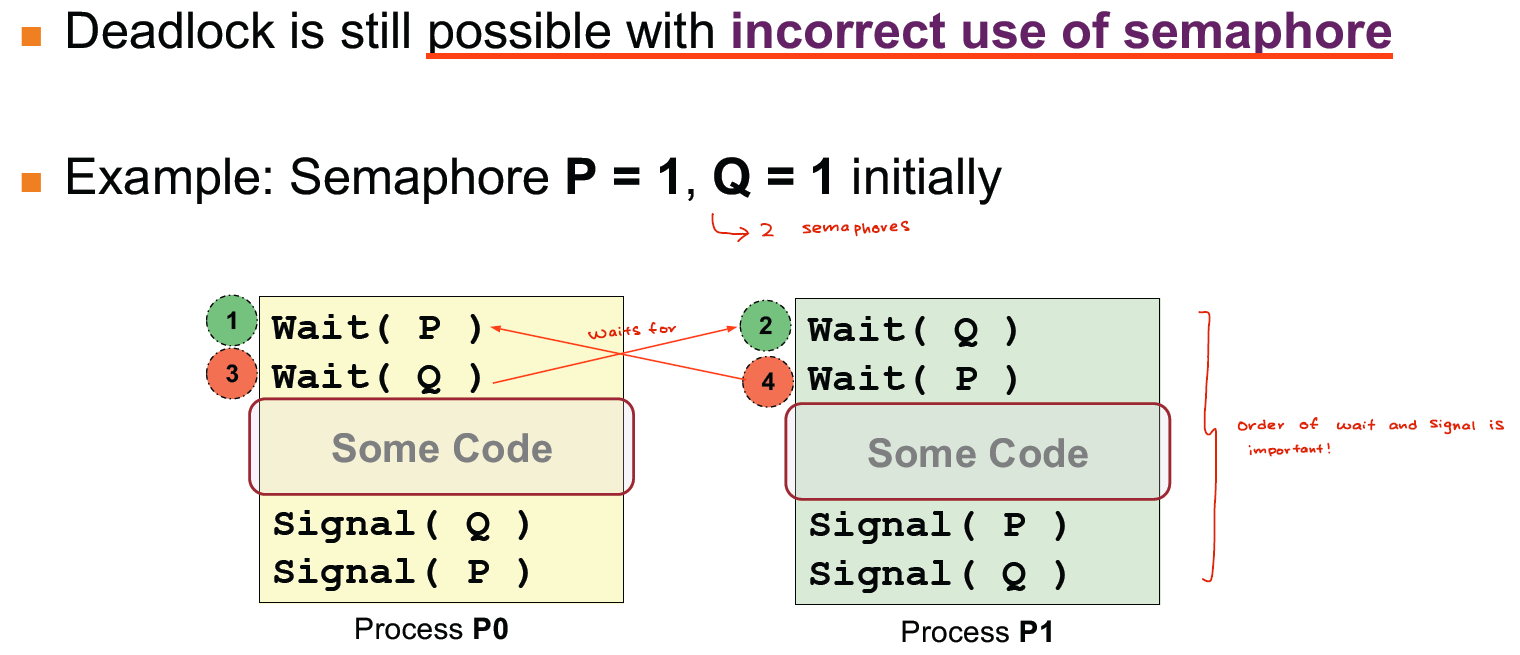
\includegraphics[width=0.8\columnwidth]{incorrect_semaphore}
        \end{center}
        %  Deadlock still possible
        %  \subsection{Classical Synchronisation Problems}
        %  \begin{itemize}
            %    \item \textbf{Producer-Consumer}: produce only if buffer not full, consume only if buffer not empty
            %    \item \textbf{Reader-Writers}: writer exclusive access, reader can share
            %    \item \textbf{Dining Philosophers}: assign partial order to the resources, establishing convention that all resources will be requested in order. E.g. label forks 1-5, and always pick up lower-numbered fork first.
            %  \end{itemize}
        %  \subsection{Synchronisation Implementations}
        %  \begin{itemize}
            %    \item POSIX semaphores
            %    \item pthread\_mutex\_t: \texttt{pthread\_mutex\_lock}, \texttt{pthread\_mutex\_unlock}
            %    \item pthread\_cond\_t: \texttt{pthread\_cond\_wait}, \texttt{pthread\_cond\_signal}, \texttt{pthread\_cond\_broadcast}
            %  \end{itemize}
        \section{Miscellaneous}
        \textbf{Process State Diagram}:
        \begin{center}
            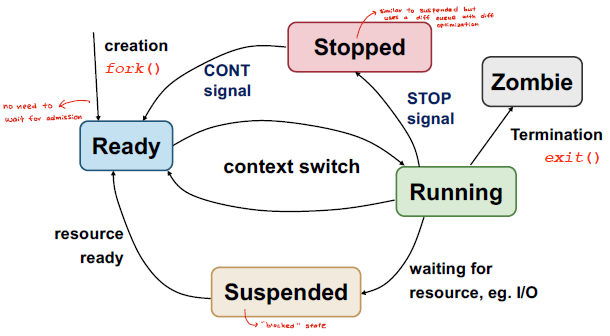
\includegraphics[width=0.7\columnwidth]{process-state-diagram}
        \end{center}
        \textbf{Priority Inversion}\\
        \begin{minipage}{\columnwidth}
            \makeatletter
            \newcommand{\@captype}{figure}
            \makeatother
            \centering
            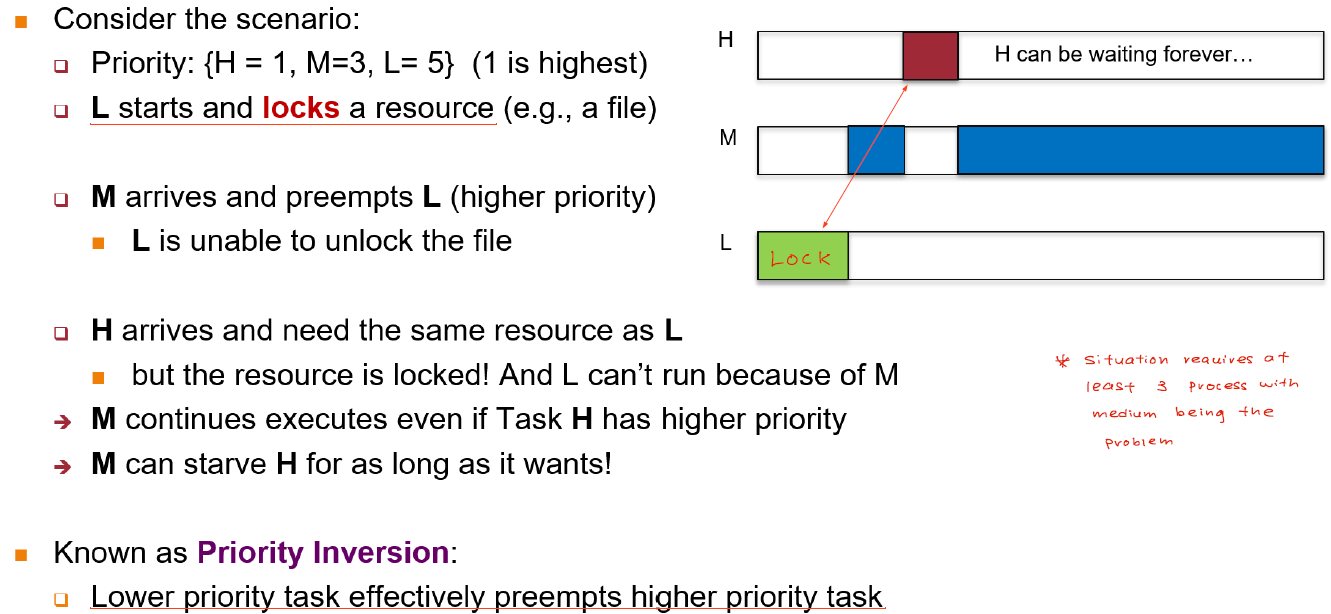
\includegraphics[width=0.7\columnwidth]{priority_inv}%
            \qquad%
            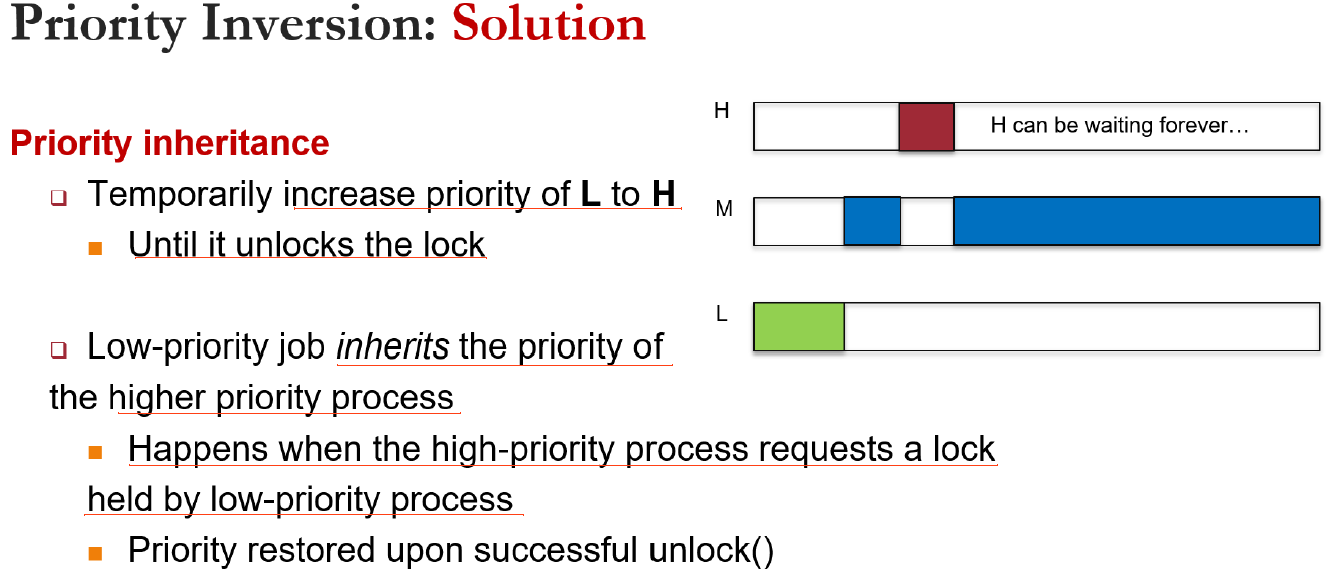
\includegraphics[width=0.6\columnwidth]{priority_inv_sol}%
        \end{minipage}
        \section{Office hours (Pre-Midterms)}
        \subsection{OS vs Kernel}
        \textbf{Kernel}:
        \begin{itemize}
            \item Essence of OS, manages and protects CPU, memory and other key resources
            \item doesn't use SYSCALLs, normal libraries and normal I/O
        \end{itemize}
        \textbf{OS}:
        \begin{itemize}
            \item Just a program with special features: deals with hardware issues, provides SYSCALLs, handles interrupts and device drivers
            \item User-friendly packaging of kernel: Includes lots of non-essential functionalities (GUI), superset of kernel
        \end{itemize}
        \subsection{Kernel mode}
        Kernel mode is the \textbf{most privileged mode of execution} in hardware which is mainly ran by the kernel. Other parts of OS use less privileged mode of execution.
        \subsubsection{Kernel mode vs Super user}
        \begin{itemize}
            \item Kernel mode is a mode of execution in hardware; when in this mode, you can execute any instruction with its fullest semantics. These privileges are reserved for the critical part of the kernel.
            \item Super-user privileges allow a certain user to manage users, files, and processes in an unrestricted manner. This removes certain OS-level restrictions, but not the hardware-level restrictions.
            \item Super user (e.g. \texttt{sudo}) $\neq$ kernel mode
        \end{itemize}
        \subsection{Return value}
        How does the return value gets accessed after the stackframe is torn down?
        \begin{itemize}
            \item \textcolor{red}{Teardown does NOT destroy anything!} Values from the function that returned still stays on stack frame until it is overwritten by other stack frames
            \item Teardown just changes the value of SP
        \end{itemize}

        \subsection{Stacks and Frames Exercise}
        \begin{center}
            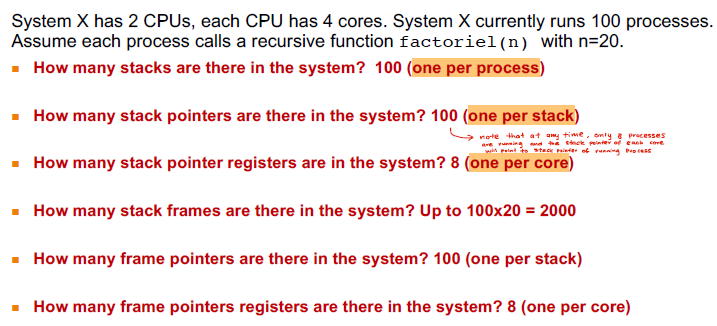
\includegraphics[width=0.8\columnwidth]{office_hours_exercise}
        \end{center}
        \subsection{Heap}
        Why dynamically allocated memory cannot use "Data" region?
        \begin{itemize}
            \item Size of data region is determined at compile time $\rightarrow$ fixed at runtime, dynamically allocated memory can be of any arbitrary size and is unknown at compile time
            \item Variables in data region lives for the duration of the program whereas dynamically allocated variables can live for as much time as the user wants (until user calls \texttt{free()})
        \end{itemize}
        \subsection{Interrupt Handling Steps}
        \begin{center}
            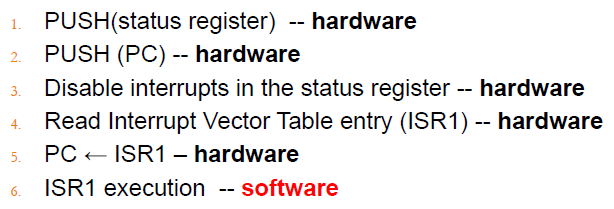
\includegraphics[width=0.8\columnwidth]{interrupt_handling}
            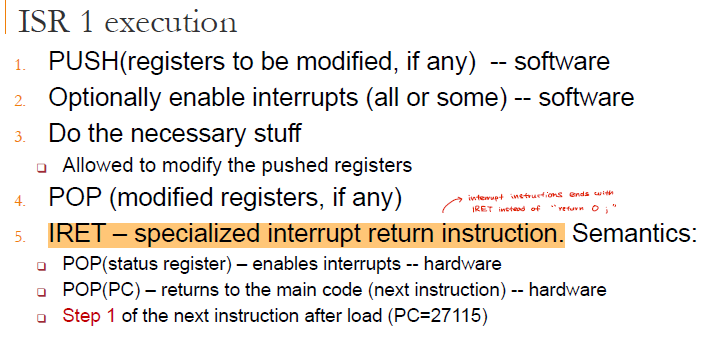
\includegraphics[width=0.8\columnwidth]{isr}
        \end{center}
        \vfill\null
        \columnbreak
        \subsection{Traps}
        Traps is an exception that is intentionally set-up (software-interrupt) and is used primarily as a means to enter kernel mode (e.g. for debugging purpose)
        \subsubsection{Traps vs Exceptions vs Traps}
        \begin{center}
            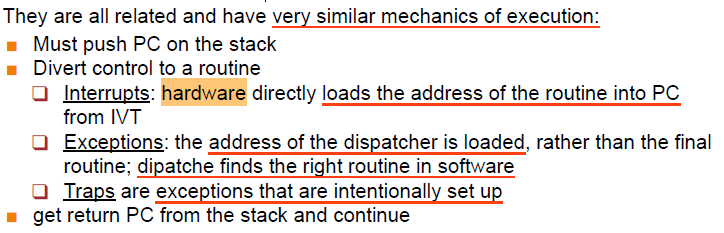
\includegraphics[width=0.8\columnwidth]{traps_exception_interrupts}
        \end{center}
        \subsection{How does fork bomb works}
        If a user runs: \mintinline{c}|while (1) { fork(); }|, it doesn't use any stack space so why would it cause problem?
        \begin{itemize}
            \item It is correct that this code does not use any stack space but since it is creating a new process and duplicating memory, there is some memory overhead (PCB, text, data, stack, heap etc.) which causes the system as a whole to run out of memory
        \end{itemize}
        \subsection{Preemptive vs Non-preemptive}
        \begin{itemize}
            \item Preemptive schedulers are needed to guarantee the responsiveness of the system
            \item Non-preemptive schedulers are used in simpler systems that do not care about responsiveness $\rightarrow$ overhead is lower
        \end{itemize}
        \subsection{Who schedule the scheduler?}
        \begin{itemize}
            \item Scheduler doesn't have to be scheduled
            \item In non-preemptive systems, when a process blocks/exits by calling a syscall, the scheduler is executed as well.
            \item For preemptive systems, the scheduler is called regularly by a timer interrupt.
        \end{itemize}
        \subsection{Scheduling Summary}
        \begin{center}
            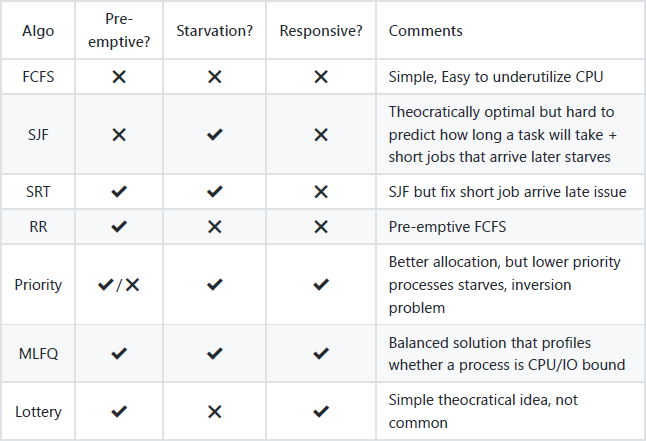
\includegraphics[width=0.7\columnwidth]{scheduling_summary}
        \end{center}
        \subsection{Are exceptions signals?}
        \begin{center}
            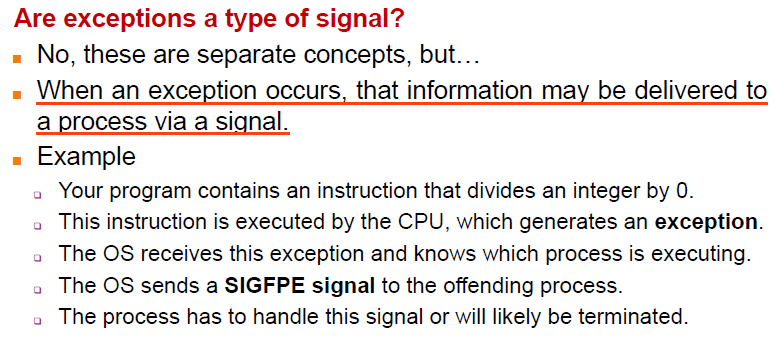
\includegraphics[width=0.7\columnwidth]{signal_exceptions}
        \end{center}
        \subsection{SRT Timer Interrupts?}
        \begin{center}
            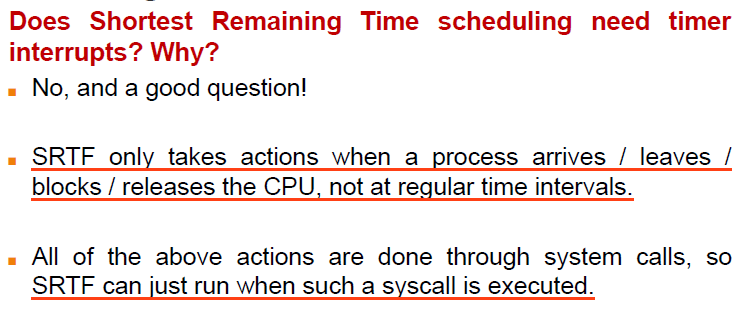
\includegraphics[width=0.7\columnwidth]{srt_timer}
        \end{center}
        \subsection{What makes lottery free of starvation?}
        \begin{center}
            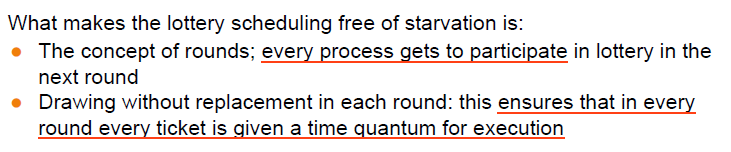
\includegraphics[width=0.9\columnwidth]{lottery_starvation_free}
        \end{center}
        \subsection{Indirect Message Passing}
        When do we use it?
        \begin{itemize}
            \item often used when it doesn't matter who
            received which message
            \item e.g. multiple clients send requests (messages) to a mailbox $\rightarrow$ mailbox buffers all the messages $\rightarrow$ multiple servers receive request from same mailbox
            \item No race conditions due to no shared data (data is copied from sender to buffer and buffer to reader) and also because OS takes care of integrity of its own message buffer
            \item Mailbox are cleaned up by the OS if process that created it crashes
        \end{itemize}
        \subsection{Kernel vs User space}
        \begin{center}
            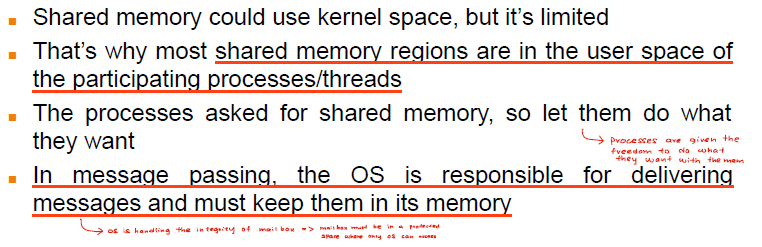
\includegraphics[width=0.9\columnwidth]{kernel_user_space}
        \end{center}
        \subsection{Kernel threads vs Actual processes}
        \begin{center}
            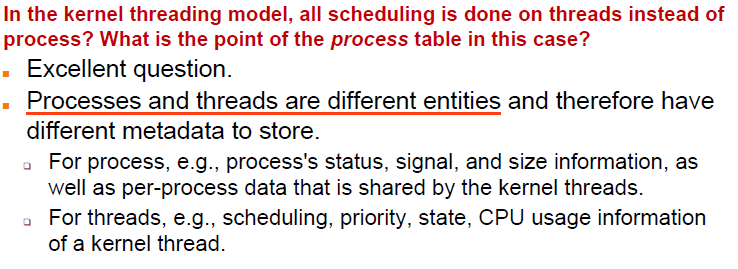
\includegraphics[width=0.9\columnwidth]{kernel_thread_vs_process}
        \end{center}
        \subsection{User thread stack}
        \begin{itemize}
            \item If OS not aware of user threads, where is the stack and register info stored?
            \item Program that manages the user thread must manage that information (likely to use heap memory to store)
            \item On top of memory management, these programs have to handle context switching, register spilling, reloading etc. on their own too
        \end{itemize}
        \subsection{Critical section properties}
        \begin{center}
            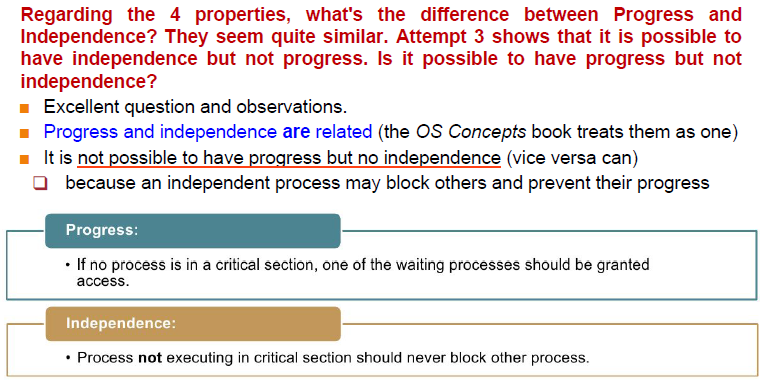
\includegraphics[width=0.9\columnwidth]{crit_section_prop}
        \end{center}
        \subsection{Uses of semaphores}
        \begin{enumerate}
            \item \textbf{Safe distancing problem}: allow only X number of processes to be running at the same time (General semaphore)
            \item \textbf{Mutex}: acts as a lock, no starvation under fair scheduling, no deadlock if used correctly, guarantees mutual exclusion (Binary semaphore)
            \item \textbf{Synchronization tool}: Execute B in \textit{$P_1$} only after A executed in \textit{$P_0$} (semaphore init to 0)
            \item \textbf{Barrier}: Only continue execution after all processes have reached barrier
        \end{enumerate}
        \columnbreak
        \section{Classical Synchronization Problems}
        \subsection{Revision: Use of Semaphores}
        \ctrimg{semaphores}
        \subsection{Producer-Consumer Problem}
        \begin{itemize}
            \item Processes share a \red{bounded buffer} of size K
            \item Producers produce items to insert in buffer when buffer is not full (< K items)
            \item Consumers remove items from buffer when buffer is not empty (> 0 items)
        \end{itemize}
        \subsubsection{Busy waiting solution}
        \ctrimg{busy_wait}
        \textit{in}: points to beginning of buffer, init to 0\\
        \textit{out}: points to end of buffer, init to 0 \\
        \textit{count}: \# of items in buffer \\
        \textit{canProduce}: init to 1 \\
        \textit{canConsume}: init to 0\\
        \textit{mutex}: Semaphore init to 1\\
        \textbf{Evaluation}: \\
        Correctly solves the problem but \red{busy-waiting} is used! e.g. 10 consumer, 1 producer, consumer will take up a lot of CPU power doing nothing and negatively impact producer
        \subsubsection{Blocking Version}
        \ctrimg{blocking}
        \texttt{wait(notFull)}: Forces producer to sleep\\
        \texttt{wait(notEmpty)}: Forces consumers to sleep\\
        \texttt{signal(notFull)}: consumer wakes up producer\\
        \texttt{signal(notEmpty)}: producer wakes up consumer\\
        * \texttt{count} no longer needed as counting semaphores \texttt{notFull} and \texttt{notEmpty} acts as count\\
        \textbf{Initial Values:}\\
        in=out=0\\
        mutex=$S(1)$, notFull=$S(k)$, notEmpty=$S(0)$\\
        \textbf{Evaluation}:\\
        Correct solves the problem and “unwanted” producer/consumer will go to sleep on respective semaphore.
        \columnbreak
        \subsubsection{Message Passing}
        \ctrimg{msg_pass}
        Elegant way of solving producer/consumer problem using OS:
        \begin{itemize}
            \item \texttt{MessageQueue} acts as buffer with \textit{K} as max elements in buffer
            \item OS blocks consumers when there are no messages
            \item OS blocks producer when buffer is full
            \item OS handles all synchronisation problems
            \item Asynchronous unless buffer full $\rightarrow$ Concurrency
        \end{itemize}
        \subsection{Readers/Writers Problem}
        \begin{itemize}
            \item Processes shares a data structure \textbf{D}:
            \begin{itemize}
                \item Reader: Retrieves information from \textbf{D}
                \item Writer: Modifies information in \textbf{D}
            \end{itemize}
            \item Writer must have exclusive access to \textbf{D}, i.e. Writer cannot be with another write nor can it be with readers
            \item Reader can access with other readers
            \item Many solutions to this problem!
        \end{itemize}
        \subsubsection{Simple Version}
        \ctrimg{simple}
        Special cases:
        \begin{itemize}
            \item $1^{st}$ reader will have to wait on \texttt{roomEmpty} to ensure that there are no more writers
            \item Last reader will have to signal to \texttt{roomEmpty} to let writers know that it is safe to write
            \item Subsequent readers after $1^{st}$ reader will wait on mutex since $1^{st}$ reader is holding mutex
        \end{itemize}
        \textbf{Evaluation}:\\
        Works but might leader to \red{starvation} for the writer! e.g. After the writer leaves, there is many readers that want to read $\rightarrow$ \texttt{roomEmpty} will never be 1 and writer can’t write any more
        \subsection{Dining Philosophers}
        \begin{itemize}
            \item 5 philosophers seated around a table
            \begin{itemize}
                \item 5 single chopsticks places between each pair of philosophers
                \item Need to acquire both chopsticks before he can eat
            \end{itemize}
            \item Want a \red{deadlock-free} and \red{starve-free} solution
        \end{itemize}
        \subsubsection{Attempt 1}
        \ctrimg{attempt_1}
        Still causes \red{deadlock} when all philosophers simultaneously take the left chopstick $\rightarrow$
        all philosophers cannot proceed since they all wait for right chopsticks\\
        \textbf{Fix Attempt}:\\
        Make each philosopher put down left chopstick if right chopstick cannot be acquired
        \begin{itemize}
            \item No deadlock but \red{livelock}!
            \item All philosophers take their left chopstick, then put it down, then take it up, put it down, ………
        \end{itemize}
        \columnbreak
        \subsubsection{Attempt 2}
        \begin{tabular}{l}
            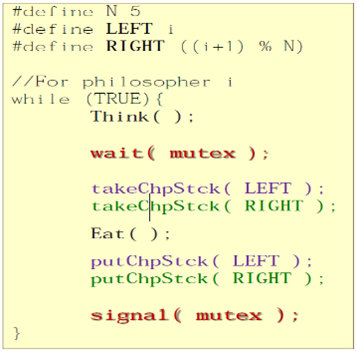
\includegraphics[width=0.30\linewidth]{attempt_2}
        \end{tabular}
        \begin{tabularx}{0.42\columnwidth}{X}
            \begin{itemize}
                \item Works but only 1 philosopher can eat at a time.
                \item Too trivial solution, \red{kills concurrency}
            \end{itemize}
        \end{tabularx}
        \subsubsection{Attempt 3}
        \begin{tabular}{l}
            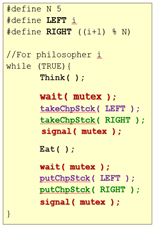
\includegraphics[width=0.23\linewidth]{attempt_3}
        \end{tabular}
        \begin{tabularx}{0.42\columnwidth}{X}
            \begin{itemize}
                \item \red{Deadlock}! Imagine the scenario where a philosopher picked up chopsticks then before he put it down another philosopher comes and tries to pick up chopstick and since he cannot pick up he will hold onto mutex lock and not allow the philosopher to put down his chopsticks
            \end{itemize}
        \end{tabularx}
        \subsubsection{Limited Eater}
        \begin{tabular}{l}
            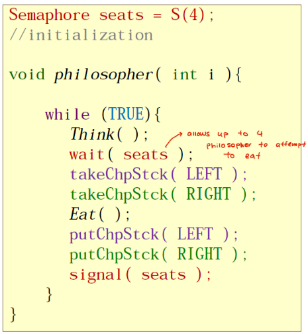
\includegraphics[width=0.25\linewidth]{limited_eater}
        \end{tabular}
        \begin{tabularx}{0.42\columnwidth}{X}
            \begin{itemize}
                \item allows only up to 4 philosophers to attempt to eat $\rightarrow$ breaks the loop $\rightarrow$
                \red{deadlock impossible}!
            \end{itemize}
        \end{tabularx}
        \subsubsection{Tanenbaum Solution}
        \begin{tabular}{l}
            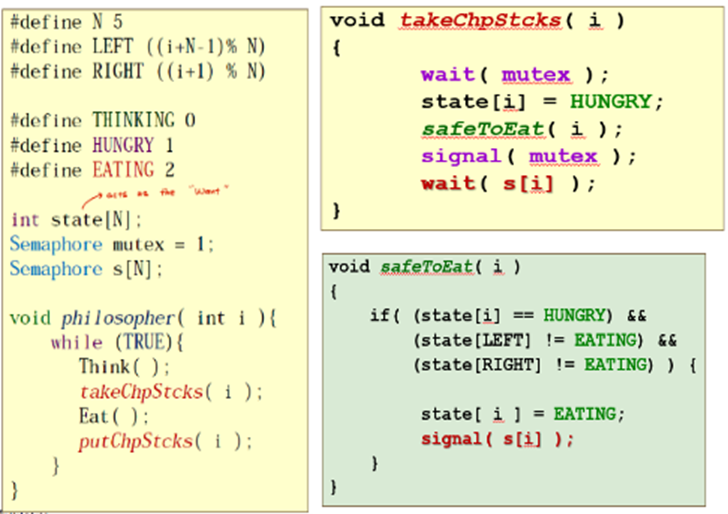
\includegraphics[width=0.45\linewidth]{tanen_1}
        \end{tabular}
        \begin{tabular}{l}
            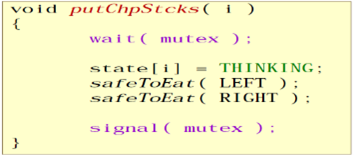
\includegraphics[width=0.4\linewidth]{tanen_2}
        \end{tabular}
        \underline{Why it works?}
        \begin{itemize}
            \item Each philosopher holds on to his own semaphore
            \item Prevents the situation where one philosopher waits on another philosopher semaphore which guarantees \red{no deadlock} (\colorbox{yellow}{starvation is possible})
            \item Once philosopher done eating then it signals its neighbours that it is safe to eat
        \end{itemize}
        \section{Memory Abstraction}
        \subsection{Memory Hardware}
        \begin{itemize}
            \item Physical memory storage:
            \begin{itemize}
                \item RAM (Random Access Memory)
                \begin{itemize}
                    \item Access latency (approximately) constant regardless of the address
                \end{itemize}
            \end{itemize}
            \item Can be treated as 1D array of AUs (addressable unit), typically 1 byte
            \item Each AU has a unique index (\red{byte addressable})
            \item 4 segments: \red{Text} and \red{Data} (fixed size after compilation), \red{Heap} and \red{stack} (size can change during runtime)
        \end{itemize}
        \subsection{Problems with unrestricted access to RAM}
        \begin{enumerate}
            \item memory hog
            \item overriding part of memory already filled
            \item allows malicious programs to access sensitive data
        \end{enumerate}
        \subsection{Calculations of Memory Address}
        \begin{itemize}
            \item After code is compiled, executable will typically contain compiled code (\red{Text region}) and \red{Global Data}.
            \item Stack and Heap are runtime structures which have \red{unknown sizes during compile time} and requires OS intervention to ensure that we can allocate memory dynamically without problems.
        \end{itemize}
        \columnbreak
        \subsection{Memory Usage: Summary}
        Generally, 2 types of data in a process:
        \begin{itemize}
            \item \textbf{Transient Data}: Valid only for limited duration e.g. function parameters, local variables live only for the duration of a function call
            \item \textbf{Persistent Data}: Valid for duration of the program or until explicitly deallocated e.g. global variables, dynamically allocated memory
            \item Both types of data sections can \textbf{grow/shrink during runtime }
        \end{itemize}
        \subsection{OS: Managing Memory}
        \begin{enumerate}
            \item Allocate memory space to new process and load process into memory
            \item Manage memory space of process
            \item Protect memory space of process from other processes
            \item Provide memory related syscalls e.g. \texttt{malloc, shm}
            \item Manage kernel memory for internal OS use (OS cannot call malloc to allocate new memory for itself!)
        \end{enumerate}
        \subsection{Memory Abstraction}
        \subsubsection{Without Memory Abstractions}
        \begin{itemize}
            \item Processes \textbf{directly uses physical addresses}
            \item Pros:
            \begin{itemize}
                \item Memory access is straightforward (fastest way of accessing memory)
                \item Address in program == Physical address
                \item No conversion/mapping required
                \item Address fixed at compile time
            \end{itemize}
            \item Cons:
            \begin{itemize}
                \item Hard to protect memory space
                \item 2 processes occupy same physical location $\rightarrow$ both processes assume their memory start at 0
            \end{itemize}
        \end{itemize}
        \subsubsection{Fix Attempt: Memory Relocation}
        Idea: Recalculate memory references during loading
        \ctrimg[0.6]{relocation}
        Problems:
        \begin{itemize}
            \item Slow loading time (relies on OS to recalculate address which \red{significantly increases load time})
            \item Not easy to distinguish pointers from normal integer constant (\red{lots of edge cases})
        \end{itemize}
        \subsubsection{Fix Attempt 2: Base + Limit Registers}
        \begin{itemize}
            \item Use a Base register (\colorbox{yellow}{part of hardware context}) as the base of all memory reference
            \begin{itemize}
                \item During compilation time, all memory references are compiled as offset from Base
                e.g. Base + 72
                \item At loading time, base register is initialized to starting address of memory space by hardware
            \end{itemize}
            \item Have another Limit register to indicate the range of memory space of current process
            \begin{itemize}
                \item Every memory access is checked against the limit to protect memory space integrity (cannot go beyond base + limit)
                \item Limit is just an \textbf{estimation} as we do not know the actual memory needed during runtime
                \item Limit is variable at runtime
            \end{itemize}
        \end{itemize}
        \ctrimg[0.6]{base\_plus\_limit}
        \underline{Problems: }
        \begin{itemize}
            \item To access address Adr:
            \begin{enumerate}
                \item Actual = Base + Adr (where Adr is the address where the program think the data is)
                \item Check Actual < Limit for validity
            \end{enumerate}
            \item Each memory access incurs addition and comparison which happens in the critical path of execution $\rightarrow$ \red{slows down execution time}
        \end{itemize}
        \underline{Pros:}
        \begin{itemize}
            \item Provides a crude memory abstraction $\rightarrow$ Address X in 2 different processes no longer share same physical location
        \end{itemize}
        \columnbreak
        \subsubsection{Logical Addresses}
        From the previous attempts, we can see that embedding actual physical address in program is a bad idea:
        \begin{itemize}
            \item does not allow address to be changed during run time as addresses are determined during compile time
        \end{itemize}
        \textbf{Solution}: \red{Logical Address}
        \begin{itemize}
            \item Logical Address == how the process views its memory space
            \item Logical Address $\neq$ Physical address in general
            \begin{itemize}
                \item Mapping from logical to physical address needed (mapping maintained by OS)
            \end{itemize}
            \item Allows each process to be a \red{self-contained}, \red{independent} logical memory space
        \end{itemize}
        \ctrimg{logical_add}
        \subsection{Contiguous Memory Management}
        Assumptions (only for contiguous memory):
        \begin{itemize}
            \item Process must be \red{in memory} (physical memory is large enough to contain $\geq$ 1 process with complete memory space), as one piece (occupies \red{contiguous memory region}), during whole execution
        \end{itemize}
        \subsubsection{Multitasking, Context Switching \& Swapping}
        \begin{itemize}
            \item To support \textbf{multitasking}: allow multiple processes in the physical memory simultaneously
            \item When memory is full: Free up memory by removing terminated processes, swapping blocked processes to secondary storage
        \end{itemize}
        \subsection{Memory Partitioning}
        \textbf{Memory Partition}: Contiguous memory region allocated to a single process
        \underline{Allocation Scheme:}
        \begin{enumerate}
            \item \red{Fixed-Size partitions}
            \begin{itemize}
                \item Physical memory split into fixed number of partitions of equal size (set to fit maximum expected size of any process)
                \item Each process will occupy any \red{ONE} of the partitions (1 process $\rightarrow$ 1 partition)
            \end{itemize}
            \item Variable-Size partitions
            \begin{itemize}
                \item Partition created based on the actual size of process
                \item OS keep track of occupied and free memory region
                \begin{itemize}
                    \item Performs splitting and merging when necessary (more complex, less fragmentation, better resource efficiency)
                \end{itemize}
            \end{itemize}
        \end{enumerate}
        \subsubsection{Fixed Partitioning}
        If a process does not occupy whole partition:
        \begin{itemize}
            \item Leftover space will be wasted (not allocatable to other processes), known as \red{Internal Fragmentation}
        \end{itemize}
        \textbf{Pros:}
        \begin{itemize}
            \item Easy to manage
            \item Fast to allocate (every partition is the same, just randomly pick a free partition)
        \end{itemize}
        \textbf{Cons:}
        \begin{itemize}
            \item Partition size need to be large enough to contain largest of processes
            \begin{itemize}
                \item Smaller process will have a lot of internal fragmentation
                \item If partition size is too small, some processes cannot run
            \end{itemize}
        \end{itemize}
        \subsubsection{Dynamic Partitioning}
        In dynamic allocation, with process creation/termination/swapping, there will be many free memory spaces known as holes. These \red{holes} are also called \red{external fragmentation} (does not belong to any partitions). \\\\
        Typically implemented using \red{LinkedList} which stores whether a \textbf{partition is occupied, start address, length of partition and a pointer to the next node}\\
        \textbf{Pros:}
        \begin{itemize}
            \item Flexible
            \item Removes internal fragmentation (size of partition is exactly what process needs)
        \end{itemize}
        \textbf{Cons:}
        \begin{itemize}
            \item Need to maintain more information in OS (how many partitions, how much memory is allocated to each partition etc.)
            \item Takes more time to locate appropriate region
            \item External Fragmentation
        \end{itemize}
        \columnbreak
        \subsubsection{Dynamic Partitioning: Allocation Algorithms}
        \begin{itemize}
            \item Assume OS maintains a list of partitions and holes
            \item 3 algorithms to locate hole of size M $\geq$ N:
            \begin{itemize}
                \item \textbf{First-Fit}
                \begin{itemize}
                    \item Take first hole that is large enough
                \end{itemize}
                \item \textbf{Best-Fit} (Minimize the wastage)
                \begin{itemize}
                    \item Find smallest hole that is large enough
                \end{itemize}
                \item \textbf{Worst-Fit}
                \begin{itemize}
                    \item Find largest hole
                \end{itemize}
                \item Split chosen hole into N and M – N
                \begin{itemize}
                    \item N will be new partition
                    \item M – N will be left over space i.e. a new hole
                \end{itemize}
            \end{itemize}
        \end{itemize}
        \subsubsection{Merging and Compaction}
        \begin{itemize}
            \item \textbf{Merging: }When occupied partition is free, try to merge with adjacent free partition to create a bigger hole
            \item \textbf{Compaction: }Move occupied partitions around to create bigger consolidated holes.\textbf{ Might not be able to do it if process has ptrs} since it might point to wrong address if shifted around. Done only when system cannot allocate partition for new process
            \item \textbf{\red{VERY TIME CONSUMING}}
        \end{itemize}
        \subsubsection{Multiple Free Lists}
        \begin{enumerate}
            \item Separate list of free holes from list of occupied partitions
            \item Keep multiple lists of different size holes
            \begin{itemize}
                \item Take hole from a list that most closely matches request size
                \item Partition size increases exponentially ($2^x$)
                \item Faster allocation
            \end{itemize}
        \end{enumerate}
        \ctrimg[0.6]{free_lists}
        \subsubsection{Buddy System}
        \begin{itemize}
            \item Popular implementation of Multiple Free Lists
            \item Buddy memory allocation provides efficient
            \begin{itemize}
                \item Partition splitting
                \item Locating good match for hole
                \item Partition de-allocation and coalescing
            \end{itemize}
            \item Idea:
            \begin{itemize}
                \item Free block split into half repeatedly
                \begin{itemize}
                    \item 2 halves form a buddy block
                \end{itemize}
                \item When both buddy blocks free, merge into bigger block
            \end{itemize}
        \end{itemize}
        \underline{Buddy System Implementation:}
        \begin{itemize}
            \item Keep array A[0…k], where $2^k$ is the largest allocatable block size
            \begin{itemize}
                \item Each array element, A[j] is a linked list which keeps track of free block(s) of size $2^j$ and each free block is indicated by their starting address
            \end{itemize}
        \end{itemize}
       	Algorithm:
        \begin{itemize}
            \item To allocate block of size $N$:
            \begin{enumerate}
                \item Find smallest S s.t $2^s\geq N$
                \item Access A[S] for free block
                \begin{enumerate}
                    \item if free block exists:
                    \begin{itemize}
                        \item remove block from free block list
                        \item allocate block
                    \end{itemize}
                    \item Else
                    \begin{itemize}
                        \item Find smallest R from S+1 to K s.t A[R] has free block B
                        \item For (R-1 to S)
                        \begin{itemize}
                            \item Repeatedly split B $\rightarrow$ A[S…R-1] has new free block
                        \end{itemize}
                        \item Goto step 2
                    \end{itemize}
                \end{enumerate}
            \end{enumerate}
            \item To free a block B:
            \begin{enumerate}
                \item Check in A[S], where $2^s$ == size of B
                \item If buddy of B is also free
                \begin{itemize}
                    \item Remove B and C from list
                    \item Merge B and C to get larger block
                    \item Repeat step 1 again with larger block
                \end{itemize}
                \item Else (buddy not free)
                \begin{itemize}
                    \item Insert B to list in A[S]
                \end{itemize}
            \end{enumerate}
            \item 2 blocks are buddy of size $2^s$ if lowest S bits of B and C are identical and bit S of B and C are different e.g. (left = 0 bit, right = 1 bit)
            \[\text{buddy} = \begin{cases}
                11\red{0}000 \\
                11\red{1}000
            \end{cases}\]
        \end{itemize}
        * Note: Buddy system \textbf{suffers from both external and internal fragmentation} but tries to minimize both
        \columnbreak
        \section{Disjoint Memory Schemes}
        We now remove one assumption - that process memory space is contiguous. They can now be in \textbf{disjoint physical memory locations} achieved using \textbf{paging}
        \subsection{Paging}
        Physical memory is split into \textbf{physical frames }and logical memory is split into \textbf{logical pages }so the same size (determined by hardware ). At runtime, pages of process are loaded into any available memory frame $\rightarrow$ logical memory can remain contiguous but physical memory can be disjoint!
        \subsubsection{Tricks to simplify translation}
        \begin{enumerate}
            \item Keep frame size as a \textbf{power of 2} (hard to deal with page size of say 97 bytes)
            \item Physical frame size == Logical frame size (\red{allows for same offset})
            \begin{itemize}
                \item For page size of $2^n$ and address of $m$ bits, to translate, we copy the last $n$ bits (offset) then for the leftmost $m$ – $n$ bits (page number) we just have to map logical address to physical frame
            \end{itemize}
        \end{enumerate}
        \subsubsection{Lookup mechanism}
        To support translation from logical to physical page, we will need a lookup table (\textbf{page table}) which \red{lives in OS memory on the RAM}.
        \ctrimg[0.55]{paging}
        \textbf{Physical add. = Frame\#} $\times$ \texttt{sizeof}\textbf{(frame) + offset}
        \subsubsection{Analysis of paging}
        \begin{itemize}
            \item \textbf{No external fragmentation: }No leftover physical memory region, every single frame can be used
            \item \textbf{Has internal fragmentation (insignificant): }when logical memory space $\neq$ multiple of page size. e.g. A process can require 1000 frames $\rightarrow$ will use up first 999 frames but last 1 may not be fully utilised
            \item \textbf{Clear separation of logical and physical address space: }allows for flexibility and simple translation
        \end{itemize}
        \subsubsection{Implementation: Pure software solution}
        OS stores page table information (using \red{pointers}) in PCB (kernel space of RAM), specifically in the memory context. However, this means that we will need 2 memory access (just for data) for memory every reference:
        \begin{enumerate}
            \item read indexed page table entry to get frame number
            \item access actual memory item
        \end{enumerate}
        * Possibly $\geq$ 2 memory access needed since code and data stored differently in modern von Neumann architecture
        \subsubsection{Paging with Hardware Support (TLB)}
        Processors have \red{TLB} (Translation Look-up Table) which is a specialized on-chip component to support paging. Typically, will have \textbf{1 TLB per core or per hardware thread.}
        \begin{itemize}
            \item Acts as \textbf{cache} (most frequently used cache) for page table entries
            \item \textbf{Very small}: 10s of entries only
            \item \textbf{Very fast: }$\le$ 1 clock cycle (\textbf{1ns}), must be fast since TLB accessed multiple times per cycle
            \item \textbf{TLB Hit: }Immediately can get physical address, skip looking up in page table
            \item \textbf{TLB Miss: }access page table in RAM (\textbf{50ns}) and update TLB
            \item Hit ratio is typically \red{99\%} for it to be effective
        \end{itemize}
        e.g. Assuming TLB hit rate = 90\%\\
        \textbf{Average memory access time }
        = P(hit) x latency(hit)+ P(miss) x latency(miss)\\
        = 0.9 x (1ns + 50ns) + 0.1 x (1ns + 50ns + 50ns)
        \begin{itemize}
            \item \textbf{Context switching:}
            \begin{itemize}
                \item upon context switch, pointer to TLB is saved
                \item TLB is flushed (\red{unless PID is saved}) so that new process will not get incorrect translation (if 2 process use same logical address) $\rightarrow$ ensures correctness, security, and safety issues
                \item TLB miss rate is high when original process resumes running
            \end{itemize}
        \end{itemize}
        \subsubsection{TLB Protection}
        Extend paging entries to include \textbf{access-right bit} and \textbf{valid bit}
        \begin{itemize}
            \item \textbf{Access-right bits}: each PTE will have { \texttt{writeable, readable, executable} } bits. e.g. page containing code should be executable and read only, page containing data should be readable and writeable
            \begin{itemize}
                \item every memory access is checked against access-right bits in hardware
            \end{itemize}
        \end{itemize}
        \begin{itemize}
            \item \textbf{Valid bit: }indicates whether page is valid to access by process
            \begin{itemize}
                \item OS sets valid bits during runtime
                \item every memory access checked against valid bit in hardware, if out of range $\rightarrow$ caught by OS
            \end{itemize}
        \end{itemize}
        \subsubsection{Page Sharing}
        Page table allows several processes to share the same physical memory frame by \textbf{pointing to same physical frame} in the PTE.\\
        Usage:
        \begin{enumerate}
            \item \textbf{Shared code page:} e.g. standard lib used by 2 processes
            \item \textbf{Implementing Copy-on-Write:} parent and child “share” pages until someone modifies the memory
        \end{enumerate}
        \subsection{Segmentation}
        \begin{itemize}
            \item So far, memory space of process is treated as a \textbf{single entity}. However, each process has multiple logical memory region with \red{different usage, permissions, lifetime, and scope}.
            \item Some regions \textbf{grow/shrink at runtime} (e.g. stack and heap) which makes it hard to achieve if whole process is 1 piece. We need to provision gaps in advance but makes it hard to check whether memory access is in-range
        \end{itemize}
        \subsubsection{Segmentation Scheme}
        Manage memory at level of \red{memory segments}:
        \begin{itemize}
            \item process now have a collection of segments which are \textbf{contiguous partitions} of the same size
            \item each memory segment has:
            \begin{itemize}
                \item \textbf{name: }for easy reference, usually translated to an index e.g. Text = 0, Data = 1 etc.
                \item \textbf{limit: }indicate exact range of segment
            \end{itemize}
            \item memory access becomes \textbf{Segment name + Offset} e.g. “Heap” + 245
        \end{itemize}
        * Within segment: contiguous. But individual segment can be anywhere in memory
        \subsubsection{Segment Table}
        To translate logical address to physical address, we maintain a \textbf{segment table} of [Base, Limit] indexed by SegID.\\
        \textbf{Physical Address = Base + Offset}, where offset < limit for valid access
        \ctrimg[0.55]{segment_table}
        \subsubsection{Hardware support}
        Since segment table is small, we can \textbf{store it directly onto the CPU register} to speed up access time
        \subsubsection{Segmentation Analysis}
        \textbf{Pros:}
        \begin{itemize}
            \item Each segment is an independent contiguous memory space which matches programmer’s view of memory
            \item Efficient bookkeeping since we can easily control each segment’s permission
            \item Segments can grow/shrink and be protected/shared independently
        \end{itemize}
        \textbf{Cons:}
        \begin{itemize}
            \item Segmentation requires variable-size contiguous memory regions which could lead to \red{external fragmentation}
            \item Copy-on-write copies entire segment
        \end{itemize}
        \subsection{Segmentation + Paging}
        Each \textbf{segment is now composed of pages} and has a page table of its own. Segments can grow/shrink by allocating/deallocating new page then add/remove to/from its page table. Checking of permissions happens in segment level instead of page level. \textbf{Copy-on-write will copy the entire segment.}
        \section{Virtual Memory}
        We remove another assumption that our physical memory is large enough to hold processes logical memory space completely. We also observe that secondary storage capacity (HDD, SSD) >> RAM capacity and some pages are accessed much more often than others. \\
        \textbf{Idea:} Extend on paging scheme and keep some pages on RAM and some pages on SSD/HDD
        \begin{itemize}
            \item \textbf{Logical address no longer restricted by physical memory}
            \item \textbf{More processes in memory: }improve CPU usage since more processes can be chosen to run on memory
            \item \textbf{More efficient use of physical memory: }RAM sort of becomes cache of frequently used pages
        \end{itemize}
        \subsection{Extended Paging Scheme}
        2 page types:
        \begin{enumerate}
            \item Memory resident: pages in physical memory
            \item Non-memory resident: pages in secondary storage
        \end{enumerate}
        Now requires an additional “\textbf{resident bit}” in PTE to indicate whether page is resident in memory. If CPU access non-resident page $\rightarrow$ \red{page fault} $\rightarrow$ OS bring page from storage to memory (\textbf{takes very long, ~ms})
        \columnbreak
        \subsubsection{Page Access using Extended Paging}
        \begin{enumerate}
            \item (Hardware) Check page table. If memory resident, done, else continue
            \item (Hardware)\textbf{ Page fault:} \red{TRAP}, pass control to OS
            \item (OS) Locate page in secondary storage
            \item (OS) Load copy of page in physical memory frame
            \item Done using \red{DMA} controller $\rightarrow$ CPU is free
            \item (OS) Update page table (set resident bit to 1)
            \item (OS) Go back to step 1 to re-execute \textbf{SAME} instruction
        \end{enumerate}
        * Steps 3 and 4 are I/O operation, process will get \textbf{blocked} and other processes can run
        \subsection{ Issues with virtual memory}
        \begin{itemize}
            \item Secondary storage access time >> physical memory access time
            \begin{itemize}
                \item \textbf{ms} vs \textbf{ns}, 5 orders of magnitude difference
            \end{itemize}
            \item If memory access results in page fault most of the time: have to constantly load non-resident pages into memory, known as \red{thrashing}
        \end{itemize}
        \subsubsection{Locality Principles}
        Thrashing is unlikely to occur in reality due to \red{Temporal} and \red{Spatial} locality. Most code spend a lot of time on relatively small part of code and only access small part of data in a given time period
        \begin{itemize}
            \item \textbf{Temporal}: Memory address used now is likely to be used again. C\textbf{ost of loading is amortized.}
            \item \textbf{Spatial}: Nearby memory addresses are likely to be used next. They are included in one page.
            \item It is however still possible for badly designed code/malicious code to behave badly
        \end{itemize}
        \subsection{How to decide who belongs in memory?}
        \textbf{Considerations:}
        \begin{itemize}
            \item Large start-up cost if large number of pages to allocate and initialize
            \item Need to reduce footprint of processes in RAM so that more processes can use physical memory
        \end{itemize}
        \subsubsection{Demand Paging}
        Start with no memory resident page and only \textbf{allocate page when there is a page fault}.\\
        \textbf{Pros:}
        \begin{itemize}
            \item Fast start-up time for new process (can just start without any page in RAM)
            \item small memory footprint
        \end{itemize}
        \textbf{Cons:}
        \begin{itemize}
            \item Process may appear \textbf{sluggish at the start} due to page faults
            \item page faults may have cascading effects on other processes (\textbf{thrashing} occurs!)
        \end{itemize}
        \subsection{Page Table Structure}
        Page Table information takes up space on physical memory space. Given modern context where logical memory is huge (can be $\geq$ 8TiB), page table will be as huge which cause a \textbf{high overhead} and \textbf{fragmentation} since it can occupy several frames.
        \subsubsection{Direct Paging}
        Keep all entries in a single table and allocate this huge page table to each process. To compute size of table:\\
        \begin{tabular}{l}
            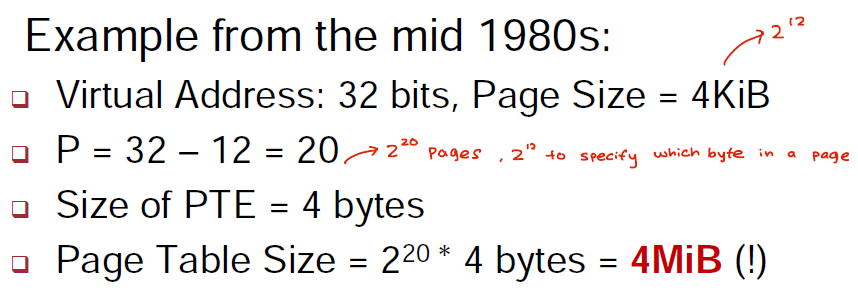
\includegraphics[width=0.4\linewidth]{direct_paging_1}
        \end{tabular}
        \begin{tabular}{l}
            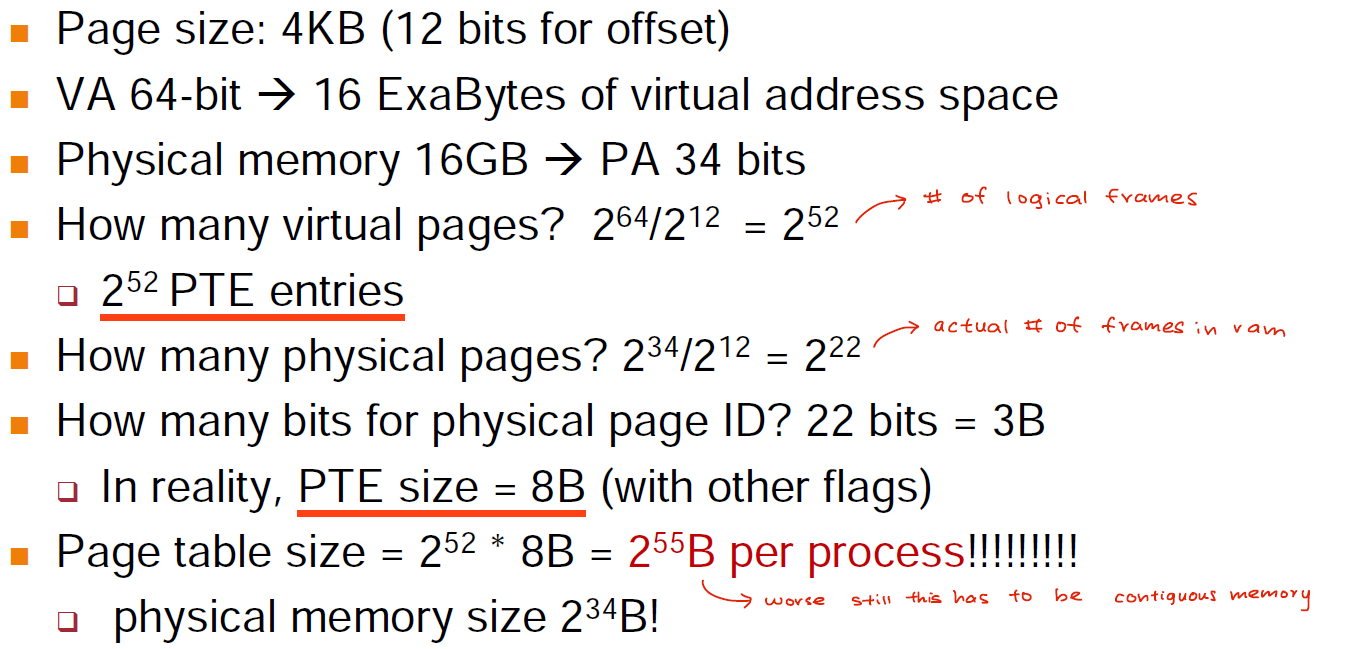
\includegraphics[width=0.53\linewidth]{direct_paging_2}
        \end{tabular}
        What’s worse is that the \red{page table must be contiguous} in OS memory to allow indexing to work (access pth entry in one memory access). Since OS memory is small, storing a table of $2^{55}$ bytes is impossible.
        \subsection{2-Level Paging}
        Further split the page table into regions and only allocate these regions when needed. We then keep a \textbf{directory} of these regions. Each table entry \textbf{points to the base address} of the next page table
        \begin{itemize}
            \item Split page table into smaller page tables (each mini page table has a number associated with it)
            \item If original page table has $2^p$ entries:
            \begin{itemize}
                \item assuming with have $2^M$ mini page tables, $M$ bits needed to uniquely identify 1 page table
                \item Each smaller page table contains $2^{(P-M)}$ entries
            \end{itemize}
            \item To keep track of smaller page table
            \begin{itemize}
                \item single page directory needed with $2^M$ indices to locate smaller page table
            \end{itemize}
        \end{itemize}
        \ctrimg[0.44]{2_level_paging}
        \columnbreak
        \subsubsection{2-Level Paging Problems}
        Requires \textbf{2 serialized memory access} (slow!) to get frame number: 1 to access directory, 1 to access page-table
        \begin{itemize}
            \item Solutions:
            \begin{itemize}
                \item \textbf{TLB}: \textbf{eliminates page-table access}, but when there is TLB miss will experience longer page-table walks (traversal of page-table in \red{hardware})
                \item \textbf{MMU (memory management unit)}: tiny cache in MMU caches frequent page directory entries to speed up page-table walks upon TLB miss. \textbf{Eliminates access to page directory.} \red{TLB for directory entries not PTEs}. Typically 1 MMU/page directory.
            \end{itemize}
        \end{itemize}
        \subsubsection{Hierarchical Page Table}
        Hierarchical Page Tables uses \textbf{indirection} design principle to reduce size of page tables.
        \ctrimg[0.9]{hierarchical_page_table}
        \subsection{Inverted Page Table}
        We want a page table that tells us \textbf{which process is using which frame}. Often used as auxiliary structure
        \begin{itemize}
            \item Keep a single mapping (only 1 per system) of physical frame to \red{<pid, page\#>}
            \item page\# may not be unique among processes
            \item pid + page\# can uniquely identify a memory page
        \end{itemize}
        \textbf{Provides:}
        \begin{itemize}
            \item \textbf{Fast lookup by frame}: answers questions like who are all the sharers of physical frame X?
            \item \textbf{Huge savings}: one table for all processes
            \item \textbf{Slow translations}: need to search the whole table to lookup page X
            \begin{itemize}
                \item Not the point of inverted page table
            \end{itemize}
        \end{itemize}
        \ctrimg[0.5]{inverted_page_table}
        \subsubsection{Page Replacement Algorithms}
        When there are no free pages during page fault, we need to evict a memory page. When page is evicted:
        \begin{itemize}
            \item \textbf{Clean page}: not modified $\rightarrow$ no need to write back
            \item \textbf{Dirty page}: modified $\rightarrow$ need to write back
        \end{itemize}
        \subsubsection{Memory Reference Strings}
        The offset does not matter when talking about page replacement, only page numbers. A sequence of page numbers is called a memory reference string.
        \subsubsection{Memory Access Time}
        $T_{access}=\left(1-p\right)\times T_{mem}+p\times T_{page_fault}$, we want to reduce $p$ since $T_{page\_fault} >> T_{mem}$
        \subsubsection{Optimal Page Replacement}
        Assuming we have knowledge of the future, we will replace the page that will not be used again for the longest period of time.
        \begin{itemize}
            \item \red{Guarantees minimum page faults} (used as benchmark)
        \end{itemize}
        \subsubsection{FIFO Page Replacement}
        Pages evicted based on loading time, \textbf{evict oldest memory page.}
        \begin{itemize}
            \item\textbf{ OS maintains queue of resident page numbers}: remove first page in queue if replacement needed, update queue during page fault
            \item \textbf{Simple to implement}: No hardware support needed
            \item \textbf{Belady’s Anomaly}: When we increase the number of frames, it leads to more page faults in FIFO algorithm.
            \begin{itemize}
                \item Due to FIFO not utilising temporal locality
                \item \red{Bad performance} in practice
            \end{itemize}
        \end{itemize}
        \columnbreak
        \subsubsection{LRU (Least recently used)}
        Replace the page that has not been used in the longest time.
        \begin{itemize}
            \item Honours Temporal Locality
            \item \textbf{Close to OPT algorithm}: predict future by mirroring the past
            \item \textbf{No Belady’s anomaly}
            \item \textbf{Difficult to implement}: need to keep track of last access time, need substantial hardware support
            \begin{enumerate}
                \item \textbf{Time counter}: A logical time counter that increments for every stored reference and is stored along with it. However, deletion is O(n) since we need to find the page with the lowest counter. We may also have overflow issues with the counter
                \item \textbf{Stack}: Maintain a stack of page numbers. When a page is referenced, we pop it out from the stack (if it’s inside) and push it to the top. For replacement, we remove the bottom most page. Hard to implement in hardware, and it’s not exactly a stack since we can pop from anywhere.
            \end{enumerate}
        \end{itemize}
        \subsubsection{Second-chance Page Replacement (Clock)}
        \textbf{Modified FIFO}. Maintain an additional reference bit for each entry: 1 means accessed since last reset, 0 means not accessed. Degenerates into regular FIFO if all referenced bit == 1.
        \begin{enumerate}
            \item maintain a circular queue of page numbers, and a pointer to the “oldest”, or victim page
            \item When we load a page entry, we set the reference bit to 0
            \item Upon accessing the page entry, we will set the reference bit to 1
            \item When a page replacement is required, we check the current victim page
            \begin{enumerate}
                \item If the reference bit is 0, we replace it
                \item Else if the reference bit is 1, we set it to 0 and move the pointer to the next page
            \end{enumerate}
            \item Repeat step 4 until a victim page with reference bit 0 is found
        \end{enumerate}
        \subsection{Frame Allocation}
        If we have N physical frame and M processes competing for these frames, how do we allocate?
        \begin{enumerate}
            \item \textbf{Equal allocation}: each process gets N / M frames
            \begin{itemize}
                \item possible to have a scenario whereby process A needs 1 page and process B needs 1,000,000 pages but both are allocated 10 pages $\rightarrow$ process B thrashes
            \end{itemize}
            \item \textbf{Proportional allocation:} each process gets $\frac{size_p}{size_{total}}\times{N}$ frames
        \end{enumerate}
        \subsubsection{Local Replacement}
        Victim page is selected among pages of the process that cause page fault
        \begin{itemize}
            \item \textbf{Constant frame allocation}: Number of frames allocated to all processes remains the same $\rightarrow$ performance is stable between runs
            \item \textbf{Insufficient Allocation}: hinders the progress of  process
            \item \textbf{Thrashing}: Limited to one process, but that single process can use up I/O bandwidth and degrade performance of other process
        \end{itemize}
        \subsubsection{Global Replacement}
        Victim page selected among pages of \red{all processes}. Possible for Process P to page fault and evict Process Q frames.
        \begin{itemize}
            \item \textbf{Self-adjustment}: Processes that need more frames can get them from other processes that need less
            \item \textbf{Inconsistent performance}: Number of frames allocated to process can differ between runs
            \begin{itemize}
                \item unfair allocation
            \end{itemize}
            \item \textbf{Cascading thrashing}: one process that thrashes will “steal” page from others, resulting in other processes also thrashing
            \item \textbf{Malicious process}: if another process does I/O and malicious process keeps thrashing, OS busy swapping frames and might not be able to schedule I/O operation, hogs up both I/O and memory bandwidth
        \end{itemize}
        \subsection{Working Sets}
        Generally, the set of \textbf{pages referenced by a process is quite constant in a period of time} due to locality. The number of page faults is minimal until the process transmits to a new locality, e.g. new function call, etc.
        \begin{itemize}
            \item Define working set window $\Delta$ which is an interval of time
            \item W(t, $\Delta$) is the set of active pages in the interval at time t
            \item We want to allocate enough frames for pages in W(t, $\Delta$) to reduce page fault
            \item Accuracy of model depends on $\Delta$
            \begin{itemize}
                \item \textbf{Too small}: miss page in locality, lots of page fault (\red{high page fault rate, low CPU utilization})
                \item \textbf{Too big}: contains page from different locality, CPU utilization will be low (\red{low page fault rate but low CPU utilization too})
            \end{itemize}
        \end{itemize}
        \ctrimg[0.5]{working_set}
        \subsection{All Page Entry Bits Thus Far}
        Access right bits, Valid Bit, Is-Memory Resident Bit, Dirty Bit, Reference Bit (for clock algo)
        \columnbreak
        \section{File Systems}
        \subsection{Motivation}
        \begin{itemize}
            \item Physical memory is \textbf{volatile}: Once you shutdown your computer, RAM is cleared
            \item Have to use external storage to store persistent information: even after restart, data still remains
            \item Direct access to storage media is \textbf{not portable}: Dependent on hardware specification and organization
            \item File system provides:
            \begin{itemize}
                \item \textbf{abstraction} on top of physical media
                \item high level \textbf{resource management} scheme: buses to read data and how we allocate memory
                \item \textbf{Protection} between processes and users: ability to isolate founds among users
                \item \textbf{Sharing} between processes and users
            \end{itemize}
        \end{itemize}
        \subsubsection{General Criteria}
        \begin{itemize}
            \item \textbf{Self-Contained}: Info on media should describe the entire organisation. Hence, can plug-and-play on another system (provided it runs on same file system).
            \item \textbf{Persistent}: Data persists beyond processes and OS
            \item \textbf{Efficient: }Good management of free \& used space + minimal overhead for bookkeeping
        \end{itemize}
        \subsection{Memory vs File Management}
        \ctrimg[0.8]{mem_vs_file}
        \subsection{File System Abstraction}
        Consists of files and directories, and provides an abstraction for accessing these.
        \subsubsection{Files}
        \begin{itemize}
            \item logical unit of information created by process
            \item essentially an abstract data type with a set of common operations
            \item Contains \textbf{data} (information structured in some way) and \textbf{metadata} (additional information associated with file)
        \end{itemize}
        \subsubsection{File Metadata}
        \ctrimg{metadata}
        \underline{File Name}
        \begin{itemize}
            \item Different FS has different naming rule (e.g. FAT32 follows 8.3 format $\rightarrow$ xxxxxxxx.(ext))
            \item Rules: length, case sensitivity, allowed special symbols and file extension (indicates file type in some FS)
        \end{itemize}
        \columnbreak
        \underline{File Type}
        \begin{itemize}
            \item OS commonly supports multiple file types
            \item Each file type has associated set of operations, possibly a specific program for processing (e.g. PowerPoint for .pptx)
            \item Common file types:
            \begin{itemize}
                \item \textbf{Regular files}: contains user information
                \begin{itemize}
                    \item ASCII files: text files, source codes, etc. Can be printed as is.
                    \item Binary files: executables \texttt{mp3, pdf} etc. Have a predefine internal structure that needs a specific program to access
                \end{itemize}
                \item \textbf{Directories}: system files for FS structure
                \item \textbf{Special files}: character/block oriented (e.g. \texttt{/dev/stdin})
            \end{itemize}
            \item \textbf{Windows}: Use file extension as file type
            \item \textbf{UNIX}: use \red{magic number} embedded at start of file
        \end{itemize}
        \underline{File Protection}
        \begin{itemize}
            \item Controlled access to information stored in file
            \item Types of access:
            \begin{itemize}
                \item Read: Retrieve information from file
                \item Write: Write/Rewrite the file
                \item Execute: Load file into memory and execute it
                \item Append: Add new information to the end of file
                \item Delete: Remove the file from FS
                \item List: Read metadata of a file
            \end{itemize}
            \item Most common approach: Restrict access base on user identity
            \begin{enumerate}
                \item Access Control List
                \begin{itemize}
                    \item list of user identity and the allowed access types
                    \item \textbf{Pros}: Very customizable
                    \item \textbf{Cons}: Additional information associated with file (overhead due to more metadata stored)
                \end{itemize}
                \item Permission Bits:
                \begin{itemize}
                    \item Classified the users into three classes: Owner (user who created file), Group (set of users who need similar access), Universe (all other users)
                    \item Note that directory permission and file permission are different (allows us to modify a file under a "read only" directory if the file has write permission)
                \end{itemize}
                \ctrimg[0.4]{perm_bits}
            \end{enumerate}
        \end{itemize}
        \underline{Operations on Metadata}\\
        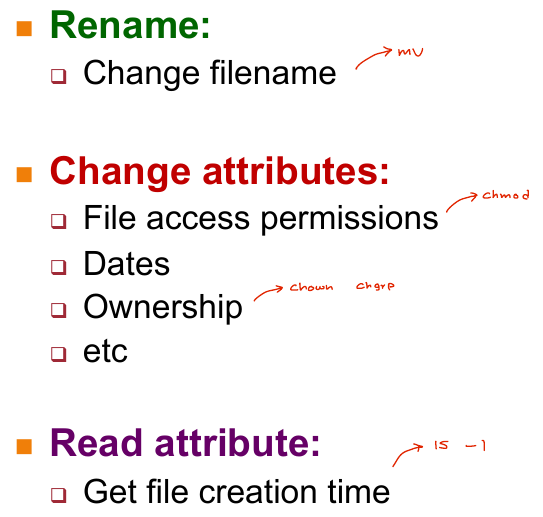
\includegraphics[width=0.35\columnwidth]{ops_on_metadata}
        \subsubsection{File Data}
        \underline{Access Methods}
        \begin{itemize}
            \item \textbf{Sequential Access} (e.g. Tape Drives): \textbf{data read in order}, starting from beginning. Cannot skip but can rewind
            \item \textbf{Random Access}: data can be \textbf{read in any order}. Either use \texttt{Read}(Offset) or \texttt{Seek}(offset). Basically a special case of direct access where 1 record == 1 byte
            \item \textbf{Direct Access}: used for files containing fixed-length records, allows random access to any record directly. Often used in databases where there is a large\# of records
        \end{itemize}
        \underline{File Operations}
        \ctrimg[0.7]{file_op}
        \subsection{Representation of Open File}
        OS provides file operations as syscalls to provide protection and allow for concurrent and efficient access. Some information will hence need to be kept by the OS:
        \begin{enumerate}
            \item \textbf{File pointer}: Current location in file
            \item \textbf{Disk location}: Actual file location on disk
            \item \textbf{Open count}: How many process has this file open. Useful to determine when to remove the entry
        \end{enumerate}
        \subsubsection{2 Table Approach}
        \begin{enumerate}
            \item \textbf{System-wide open-file table} (Kept on OS Memory on RAM)
            \begin{enumerate}
                \item Keeps track of open files in the system
                \item If same process opens the same file twice, or two processes open the same file, there will be \red{two separate entries} in the open file table (doing different things to file at different offsets $\rightarrow$ need different fd)
                \item If one process opens a file then \textbf{forks}, \red{only one entry} in open file table
            \end{enumerate}
            \item \textbf{Per-process open-file table}
            \begin{enumerate}
                \item Keeps track of open files for a process, also known as \textbf{file descriptors}
                \item Each entry points to a system-wide table entry
                \item If one process opens a file then forks, there will be two fds pointing to the same system-wide table entry. They will thus share the same offset
                \item If the same process open the same file multiple times, there will be multiple entries in the per-process file table
                \item \textbf{Default file descriptors: (1) STDIN (2) STDOUT (3) STDERR}
            \end{enumerate}
        \end{enumerate}
        \subsection{Directory}
        Helps to provide a logical grouping of files and keep track of files.\\\\
        \begin{tabular}{l}
            \textbf{Single Level}\\
            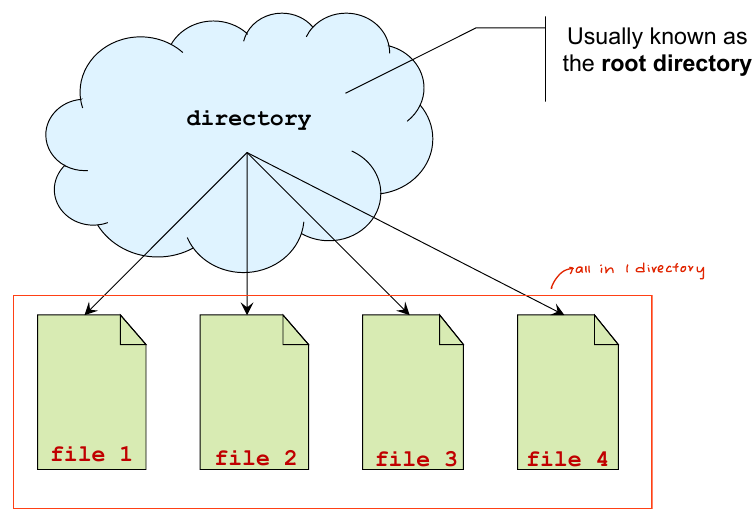
\includegraphics[width=0.44\linewidth]{single_level}
        \end{tabular}
        \begin{tabular}{l}
            \textbf{Tree Structure}\\
            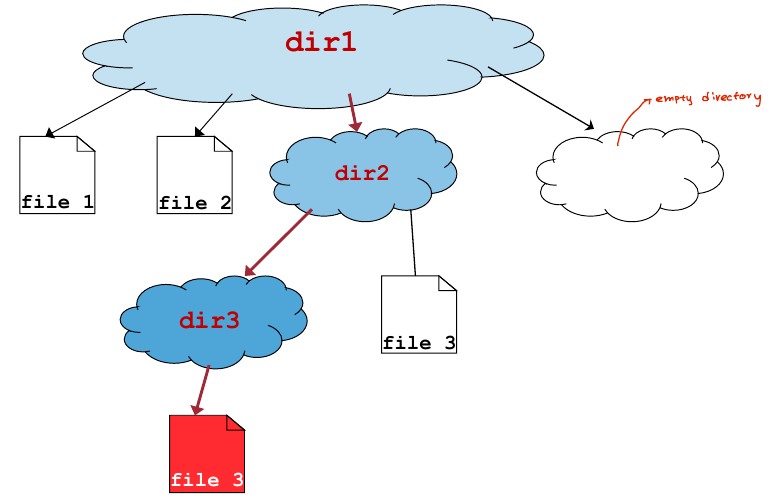
\includegraphics[width=0.44\linewidth]{tree_structure}
        \end{tabular}
        \newline
        \begin{tabular}{l}
            \textbf{DAG}\\
            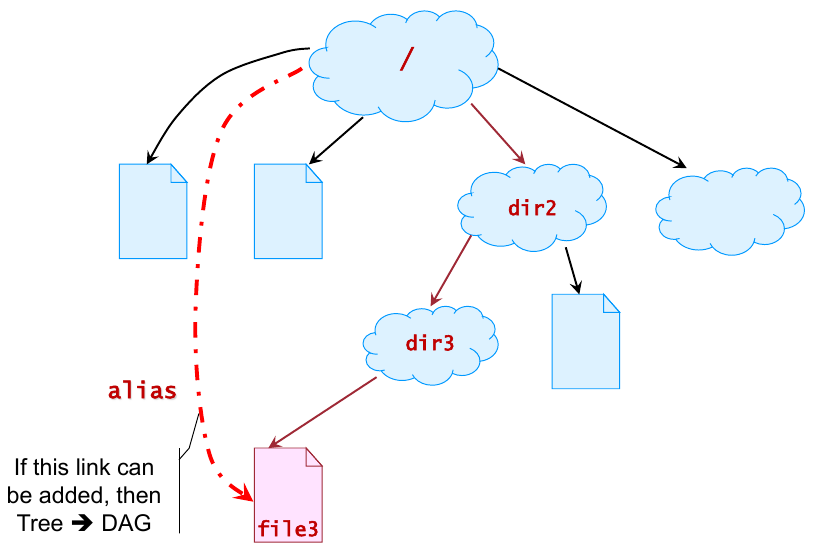
\includegraphics[width=0.44\linewidth]{dag}
        \end{tabular}
        \begin{tabular}{l}
            \textbf{General Graph}\\
            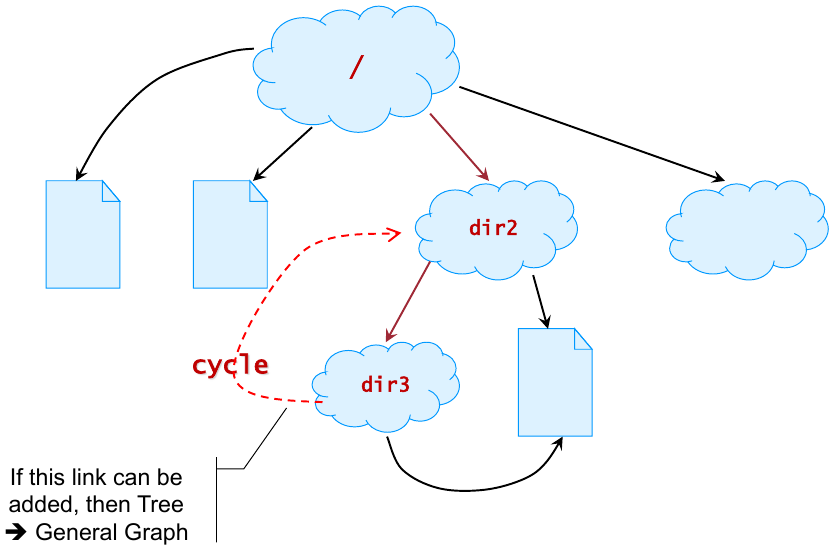
\includegraphics[width=0.44\linewidth]{general_graph}
        \end{tabular}
        \subsubsection{Tree Structure}
        \begin{itemize}
            \item Directories can contain directories: Forms a tree structure where files are leaves
            \item \textbf{Absolute Pathname}: Refer to file by path from Root
            \item \textbf{Relative Pathname}: Refer to file from \textbf{current working directory}
        \end{itemize}
        \subsubsection{DAG}
        \begin{itemize}
            \item To get a DAG, we must be able to "skip" level, i.e. share a file/directory such that it appears in multiple directories but refer to same copy of actual content
            \item \textbf{Hard links}: Directories \textit{A} and \textit{B} have separate pointers to file \textit{F}. \red{Only works with files}
            \begin{itemize}
                \item Pros: Low overhead, only pointers are added in directory (only take up directory space)
                \item Cons: Deletion problems - if only one of $A$ or $B$ deletes the file, the data remain. To completely delete data, we will need to delete all reference to the file.
                \item \texttt{ln} command in UNIX
            \end{itemize}
            \item \textbf{Symbolic Links}: Directory $B$ creates a special link file $G$ that contains path name of $F$. When $G$ is access we access $F$ instead.
            \begin{itemize}
                \item Pros: Simple deletion. When $B$ is deleted, delete $G$ but not $F$. If $A$ is deleted, $F$ is gone, $G$ remains but does not work
                \item Cons: Larger overhead - link file take up actual disk space
                \item \texttt{ln -s} command in UNIX
            \end{itemize}
        \end{itemize}
        \subsection{General Graph}
        Created when tree has a cycle. Possible in UNIX but not desirable.
        \begin{itemize}
            \item Hard to traverse: Need to prevent infinite loops
            \item Hard to determine when to remove file/directory
        \end{itemize}
        \subsection{I/O: Disk Structure}
        \begin{tabular}{l}
            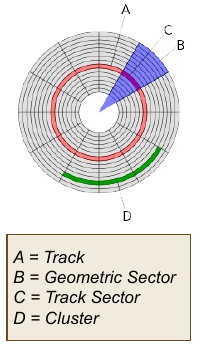
\includegraphics[width=0.25\linewidth]{disk}
        \end{tabular}
        \begin{tabularx}{0.42\columnwidth}{X}
            \begin{itemize}
                \item \textbf{Track}: One ring around disk. One disk can have many tracks of different radii
                \item \textbf{Geometric Sector}: Sector of a track
                \item \textbf{Disk Head}: Stick thingy that moves above the disk. Transforms disk's magnetic field into electrical currents
                \item \textbf{Rotation}: typically 3600/5400/7200 RPM
                \item \textbf{Seek}: Shifting of the head to change track
                \item \textbf{Time taken to access data on dis}k: Seek time + Rotational Delay + Transfer delay
            \end{itemize}
        \end{tabularx}
        \section{File System Implementation}
        File systems are stored on storage media (e.g. HDD, CD/DVD, SRAM/DRAM). To the OS, disk sectors are treated as a 1-D array of logical blocks, usually 512 bytes to 4KiB. The mapping between the logical block and sectors is \textbf{hardware dependent}
        \subsection{Disk Organization}
        \begin{itemize}
            \item \textbf{Master boot record (MBR)}: Found at sector 0. Contains:
            \begin{itemize}
                \item Simple Boot Code
                \item Partition Table (tells where partitions start and end)
            \end{itemize}
            \item \textbf{Partitions}: Each partition can contain an independent file system. Contains:
            \begin{enumerate}
                \item OS Boot-up information
                \item Partition details: total number of blocks, number and location of free disk blocks
                \item Directory Structure
                \item Files Information
                \item Actual file data
            \end{enumerate}
        \end{itemize}
        \subsection{File Implementation}
        In the process of allocating file data, we need to keep track of logical blocks, allow efficient access and utilize disk space efficiently. There will be \red{internal fragmentation} when file size $\neq$ multiple of logical blocks
        \subsubsection{Contiguous Allocation}
        Allocate consecutive disk blocks to a file\\
        \textbf{Pros:}
        \begin{itemize}
            \item Simple to keep track - each file only need starting block\# + length
            \item Fast access: just need to seek first block
            \item Good for WORM (write once read many) drives e.g. CD-ROM
        \end{itemize}
        \textbf{Cons:}
        \begin{itemize}
            \item \red{External Fragmentation}: Think of each file as variable size partition. After a lot of creation/deletion, disk can have many small "holes".
            \item File size need to be specified in advance
        \end{itemize}
        \subsubsection{Linked List}
        Maintain disk blocks as linked list. Each block stores ptr to next block and actual file data. File information stores first and last disk block (to support fast append operations)\\
        \textbf{Pros:}
        Solve fragmentation problem\\
        \textbf{Cons:}
        \begin{itemize}
            \item Random access is very slow
            \item Less usable space: part of disk block used to store pointer
            \item Less reliable: fails if 1 pointer is incorrect
            \item possible to create circular linked list!
        \end{itemize}
        \subsubsection{Linked List V2}
        Same as Linked List but we move all ptrs into a file allocation table (FAT) \red{in memory}.
        \begin{itemize}
            \item \textcolor{green}{\textbf{Faster access}}: Traversal now happens in memory instead of disk
            \item \red{Takes up space}: Fat keeps track of all disk blocks in partition. Huge when disk is large, consuming memory space
        \end{itemize}
        \subsubsection{Indexed Allocation}
        Each file has an index block which stores an array of disk block addresses/ IndexBlock[N] == $N^{th}$+1 block address. Each block now can either store data or the array.\\
        \textbf{Pros:}
        \begin{itemize}
            \item \textbf{Lesser memory overhead}: only index block of opened file needs to be in memory
            \item \textbf{Fast direct access}: No need traverse
        \end{itemize}
        \textbf{Cons:}
        \begin{itemize}
            \item \textbf{Limited Max File Size}: Max number of blocks == Number of index block entries
            \item \textbf{Index block overhead}
        \end{itemize}
        \underline{Variations}
        \begin{itemize}
            \item Exists other schemes to allow larger file size
            \item \textbf{Linked scheme}: Keep linked list of index blocks
            \begin{itemize}
                \item Each index block contains pointer to next index block
            \end{itemize}
            \item \textbf{Multilevel index}: similar idea to multi-level paging
            \begin{itemize}
                \item N level index blocks points to a number of N + 1 level index blocks
                \item UNIX I-Node uses this idea: 12 direct pointers, 1 single indirect block, 1 double indirect block, 1 triple indirect block
            \end{itemize}
        \end{itemize}
        \columnbreak
        \textbf{I-Node Structure}
        \ctrimg{inode}
        \subsection{Free Space Management}
        To perform file allocation, we need to know which disk blocks are free/not free
        \subsubsection{Bitmap}
        Each block is represented by 1 bit. 1 == free, 0 == occupied\\
        \textbf{Pros:} Easy to manipulate: use bit operations to find first free block or n-consecutive free blocks\\
        \textbf{Cons:} Need to keep in memory for efficiency reason
        \subsection{Linked List}
        Use a linked list of disk blocks containing number of free disk block numbers and a pointer to next free space disk block\\
        \textbf{Pros:} Easy to locate free block, only first pointer needs to be in memory (memory efficient) though we can cache other blocks for efficiency\\
        \textbf{Cons:} High overhead as we are storing free block numbers in data block. Can be mitigated by storing free blocks list in free blocks instead.
        \subsection{Directory Structure}
        Main task of directory structure is to provide some \textbf{mapping between file name and file information} and to keep track of files in a directory. To use a file, have to use the syscall \texttt{open} which locates file information using pathname + filename. Sub-directory is usually store as \red{file entry} with a special type in a directory
        \subsubsection{Linear List}
        \ctrimg[0.63]{linear_list}
        \subsubsection{Hashtable}
        \ctrimg[0.63]{hashtable}
        \subsubsection{File Information}
        \ctrimg[0.63]{file_info}
        \subsubsection{File System in Action}
        \begin{tabular}{l}
            \textbf{File Creation}\\
            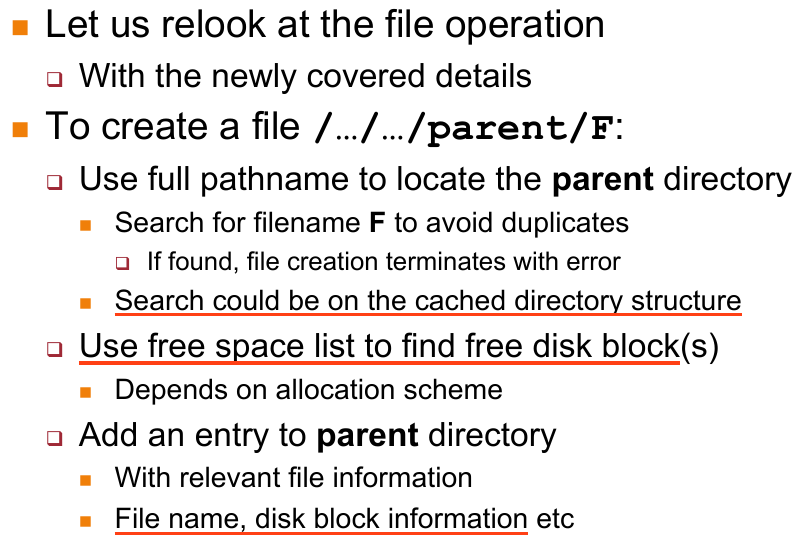
\includegraphics[width=0.44\linewidth]{create_file}
        \end{tabular}
        \begin{tabular}{l}
            \textbf{File Opening}\\
            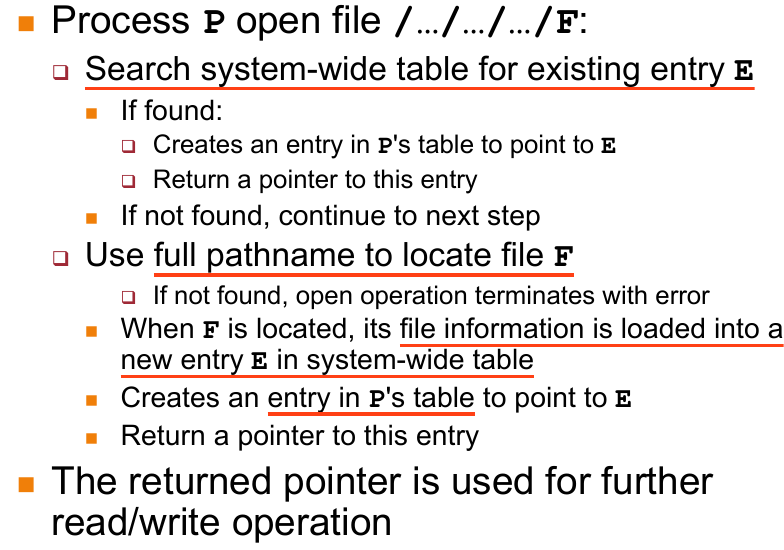
\includegraphics[width=0.44\linewidth]{open_file}
        \end{tabular}
        \subsection{Disk I/O Scheduling}
        Time taken to perform read/write operation\\
        = \textbf{[Seek Time]  + [Rotational Delay] + [Transfer Time]}
        \begin{itemize}
            \item \textbf{Seek time}: time taken to position disk head over correct track (typically \red{2ms to 10ms})
            \item \textbf{Rotational Latency}: time taken to wait for desired sector to rotate under disk head (\red{4ms to 12.5ms per rotation}, average is $\frac{1}{2}$ of 1 full rotation time)
            \begin{itemize}
                \item Worst case: Sector just passed head, wait 1 full rotation
                \item Best case: Sector is just before head. 0 rational delay
            \end{itemize}
            \item \textbf{Transfer delay}: time taken to transfer sector, function of Transfer size / Transfer rate, typically takes $\mu$s which is \red{3 orders of magnitude faster} than previous 2 delays
            \item Possible to suffer from same problems as normal scheduling, e.g. starvation when running SSF
        \end{itemize}
        \subsubsection{Scheduling Algorithms}
        \begin{itemize}
            \item \textbf{FCFS}: cannot change sequence by changing arrival time
            \item \textbf{Shortest Seek First (SSF)}
            \item \textbf{SCAN}: Bi-directional, go from innermost to outermost then back to innermost. Much like a lift.
            \item \textbf{C-SCAN}: Unidirectional, Go from outermost to innermost then reset
        \end{itemize}
        \section{File System Case Studies}
        \subsection{MS FAT File System}
        \ctrimg[0.7]{MS_FAT}
        \subsubsection{File Data and FAT}
        File Data is allocated to a number of data blocks/clusters and allocation info is kept as a Linked List with pointers kept in FAT. \textbf{FAT is \red{entirely} cached in RAM} to facilitate linked list traversal and there is \textbf{1 entry in FAT table per data block/cluster} (may not be same size as physical block)\\
        \underline{FAT Entry Values}\\
        \begin{enumerate}
            \item FREE code: block is unused
            \item Block number of next block
            \item EOF code: NULL ptr
            \item BAD block: block is unusable e.g. disk error due to scratches on disk. Found out using a checksum
        \end{enumerate}
        \underline{Directory}
        \begin{itemize}
            \item Special type of \red{file}
            \item Root directory stored in a special location, other directories stored in data blocks
            \item Each file or subdirectory within the folder is represented by a \textbf{directory entry}
        \end{itemize}
        \underline{Directory Entry}\\
        Each entry has fixed-sized of 32 bytes\\
        \textbf{Contains:}
        \begin{itemize}
            \item Name + Extension (11 bytes)
            \begin{itemize}
                \item Limited to 8 + 3 characters (8 char for file name, 3 characters for file ext.)
                \item First byte may have meaning (e.g. deleted, end of directory entries, parent directory)
            \end{itemize}
            \item Attributes e.g. read-only, is-directory/file flag, hidden-flag (1 byte)
            \item Reserved: for future use (10 bytes)
            \item Creation date (2 bytes) + Time (2 bytes)
            \begin{itemize}
                \item Year range: 1980 -- 2107
                \item Accurate to $\pm$ 2 seconds
            \end{itemize}
            \item First Disk Block Index (2 bytes)
            \begin{itemize}
                \item Disk block index is 12, 16 and 32 bits for FAT12, FAT16 and FAT32 respectively
                \item For FAT32 lower half is stored
            \end{itemize}
            \item File Size in bytes (4 bytes)
        \end{itemize}
        \ctrimg[0.7]{FAT_Illustration}
        \subsubsection{Tracing Process}
        \begin{enumerate}
            \item Use first disk block number stored in directory entry to find the starting point of the linked disk blocks
            \item Use FAT to find out the subsequent disk blocks number, terminated by EOF
            \item Use disk block number to perform actual disk access on the data blocks
        \end{enumerate}
        \subsubsection{Common Tasks}
        \ctrimg[0.65]{FAT_common_task}
        \subsubsection{Variants: FAT12, FAT16, FAT32}
        As storage gets larger, we want to be able to support larger hard disk as a single partition
        \begin{itemize}
            \item \textbf{Disk Cluster}:
            \begin{itemize}
                \item Instead of using a single disk block as the smallest allocation unit, we \red{use a number of contiguous disk block} as smallest allocation unit
            \end{itemize}
            \item \textbf{FAT Size}:
            \begin{itemize}
                \item Bigger FAT $\rightarrow$ More disk block/cluster $\rightarrow$ More bits to represent each disk block/cluster
                \item Existing variants: FAT12, FAT16, FAT23
            \end{itemize}
            \item Generally cluster size + FAT size determines largest usable partition
            \ctrimg[0.5]{fat_example}
            * Actual size is actually a little lesser (due to special values like EOF, FREE etc.) which reduces total number of valid block indices
        \end{itemize}
        \subsubsection{Cluster Size Tradeoff}
        \begin{itemize}
            \item Larger cluster size $\rightarrow$ larger usable partition
            \item However, larger cluster size also leads to \red{larger internal fragmentation}
            \item On FAT32 there are also further limitation: 32-bit sector count (limited partition size), but only 28 bit is used in the disk block/cluster index
        \end{itemize}
        \subsection{Long File Name Support}
        In original FAT, we can only have up to 8 characters as file name.
        \begin{itemize}
            \item \red{Virtual FAT (VFAT)} allows for filenames up to \textbf{255 characters}
            \item To support for additional characters, we use \textbf{multiple directory entries}.
            \begin{itemize}
                \item Use previously invalid \textbf{file attribute} so non-VFAT applications can ignore additional entries
                \item Use first byte to indicate sequence
            \end{itemize}
            \item Keep 8+3 short version for backward compatibility
        \end{itemize}
        \ctrimg{vfat}
        \subsection{Linux Ext2}
        The layout of the file system is now slightly different. Blocks (correspond to one or more disk sectors) are grouped into block groups and each file/directory is describes by a single special structure called \textbf{I-Node} (Index Node), containing file metadata and data block addresses
        \ctrimg[0.7]{inode_fs}
        \begin{itemize}
            \item \textbf{Superblock}: Describes the whole file system, e.g. Total I-Nodes number, I-Nodes per group, Total disk blocks, Disk Blocks per group etc. Duplicated in each block group for redundancy
            \item \textbf{Group descriptors:} Describe each of the block group, e.g. number of free disk blocks and I-Nodes per group, location of bitmap etc. Duplicated in each block group for redundancy.
            \item \textbf{Block Bitmap:} Keeps track of usage status of blocks in this block group (1 = Occupied, 0 = Free)
            \item \textbf{I-Node Bitmap:} Same as Block bitmap but for I-Nodes
            \item \textbf{I-Node table:} Array of I-Nodes in this block group\\
        \end{itemize}
        \begin{tabular}{l}
            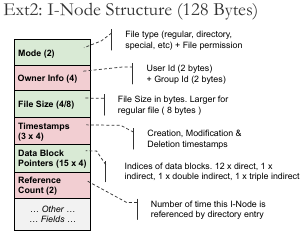
\includegraphics[width=0.44\linewidth]{inode_structure}
        \end{tabular}
        \begin{tabular}{l}
            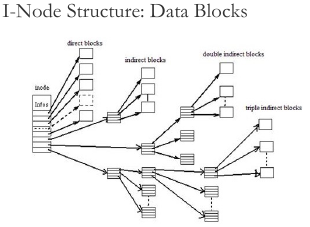
\includegraphics[width=0.44\linewidth]{inode_data}
        \end{tabular}
        \\* Note that file size \textbf{does not include file's metadata}, only includes the size of file content only
        \columnbreak
        \subsubsection{I-Node Data Block Example}
        \ctrimg[0.7]{inode_example}
        \subsubsection{Directory Structure}
        A directory is just another file. Within this file, the
        data blocks form a "linked list" (allows for variable length $\rightarrow$ name can be variable length) of directory entries for files and subdirectories within the directory.
        \begin{enumerate}
            \item I-Node number for this file or subdirectory. 0 is
            used to indicate unused entry
            \item Size of this directory entry, so we can traverse to
            the next entry
            \item Length of the name
            \item Type: file, subdirectory or special
            \item Name of file/subdirectory (up to 255) characters\\
        \end{enumerate}
        \begin{tabular}{l}
            \includegraphics[width=0.44\linewidth]{directory_entry}
        \end{tabular}
        \begin{tabular}{l}
            \includegraphics[width=0.44\linewidth]{inode_full}
        \end{tabular}
        \subsubsection{Tracing Process}
        \ctrimg[0.7]{inode_trace}
        \subsubsection{Common Tasks}
        \ctrimg[0.7]{inode_common_task}
        \columnbreak
        \subsubsection{Symbolic Link vs Hard Link}
        \begin{itemize}
            \item \textbf{Hard Link: } (can have different file names)
            \begin{enumerate}
                \item Create new directory entry in B with same I-Node number as $X$ in A
                \item Update X I-Node's reference count
                \item For deletion, decrement the reference count, then when it goes to 0, perform actual deletion
            \end{enumerate}
            \item \textbf{Symbolic Link:}
            \begin{enumerate}
                \item Create a new file $Y$ in directory $B$, i.e. new $Y$ I-Node + new directory entry for $Y$
                \item Store pathname of file $X$ in file $Y$ , i.e. that is
                the file content
                \item As only pathname is stored, the link can be easily invalidated, e.g. via name changes, deletion, etc.
            \end{enumerate}
        \end{itemize}
        \ctrimg[0.55]{links}
        \section{Process involved in calling \texttt{ls}}
        \begin{enumerate}
            \item At first, the shell/terminal starts off in the \textbf{blocked} state since it is just waiting for the user input and has nothing else to do
            \item Once the user presses "l", an interrupt is fired which calls the appropriate \textbf{interrupt handler} (e.g. 3) using the \textbf{interrupt vector table} (IVT)
            \item This in turns calls a \textbf{keyboard handler} code which is a piece of code pre-compiled in memory
            \begin{itemize}
                \item Process of executing interrupt handler, loading in IVT and running handler code is \textbf{fully done in hardware}
            \end{itemize}
            \item Since it is likely a process X was interrupted, we would \textbf{need to save X's context} (e.g. registers, memory context etc.) into the hardware context in the PCB of x
            \item This process repeats for each character entered into the command line
            \item Once user completes command and presses "enter", the interpreter could be in 1 of 3 states:
            \begin{enumerate}
                \item \textbf{Ready}: Waiting to be scheduled
                \item \textbf{Running}: Child spawned and running command
                \item \textbf{Blocked}: Parent waiting for child to finish execution
            \end{enumerate}
            \begin{tabular}{l}
                \includegraphics[width=0.40\linewidth]{shell}
            \end{tabular}
            \begin{tabular}{l}
                \includegraphics[width=0.48\linewidth]{fork}
            \end{tabular}
            \item Effect of fork?
            \begin{itemize}
                \item Save CPU register which contains ptr to root of page table
                \item No need to save: TLB, caches, process data, process page table, frames of pages
            \end{itemize}
            \item $\text{PCB}_{\text{child}}$ of the spawned child would contain a copy of the parent's PCB. The copying can be done in 2 ways:
            \begin{enumerate}
                \item \textbf{"Hard way"}: Actually allocate new frames for the copied process upon process creation
                \item \textbf{"Copy-on-write"}: Employs laziness and only allocate new frames when any process writes to data
            \end{enumerate}
            \item Memory context of the processes will contain both Page Table (incur internal fragmentation due to paging, where page size == physical frame size) and TLB (makes use of temporal and spatial locality)
            \item Child now enters the scheduling queue where it could either be in:
            \begin{enumerate}
                \item \textbf{New}: Freshly forked child
                \item \textbf{Ready}: in the queue waiting to be scheduled
            \end{enumerate}
            \item While waiting for the child, the parent is blocked which causes its hardware context to be saved so that other processes can run
            \begin{itemize}
                \item Registers are actually pushed onto the stack due to efficiency (faster to push all register to stack in a single instruction vs copying register value one by one into PCB)
            \end{itemize}
            \item We now have to replace the memory content of shell process with ls process by bringing executable of ls into memory
            \item After child is done executing, it informs parents through: (1) library call, (2) syscall (3) signal
        \end{enumerate}
        \columnbreak
        \section{QnA}
        \subsection{OS Abstractions and Protections}
        \textbf{Process (CPU Time)}
        \begin{itemize}
            \item \textbf{Abstraction}: illusion that process executes on CPU all the time
            \item \textbf{Protection}: Execution context of each process is isolated from each other
        \end{itemize}
        \textbf{Memory Management}
        \begin{itemize}
            \item \textbf{Abstraction}: illusion that process owns the entire memory space
            \item \textbf{Protection}: Memory space of each process are mapped to different physical address, isolating them from each other
        \end{itemize}
        \textbf{File Management}
        \begin{itemize}
            \item \textbf{Abstraction}: Files is a single contiguous logical entity
            \item \textbf{Protection}: Files can only be opened through system call, OS can prevent files from being opened for incompatible operations
        \end{itemize}
        \subsection{Swap Files}
        \textbf{Should swap files be considered as normal files?}
        \begin{itemize}
            \item No. They require contiguous chunk of memory to speed up paging. Normal files may have their data stored at different parts of the secondary storage.
        \end{itemize}
        \textbf{Relationship between Page size and Cluster Size}
        \begin{itemize}
            \item Page size should be multiple of cluster size to allow efficient swapping of pages.
        \end{itemize}
        \textbf{Should swap file be system-wide or per-process?}
        \begin{itemize}
            \item System wide. Allows OS to allocate a contiguous chunk of secondary storage for it at the start. Also it is hard to predict user usage if we use per-process swap which makes allocation of memory in storage difficult.
        \end{itemize}
        \subsection{Virtual Memory}
        \textbf{Can threads from same process share same page table?}
        \begin{itemize}
            \item Yes. Use the same virtual memory space as the process.
        \end{itemize}
        \textbf{Is the memory address returned by \texttt{shmat()} likely to be at boundary of memory page?}
        \begin{itemize}
            \item Yes. We need to set the translation (i.e. frame number) to the shared region different from other memory locations.
        \end{itemize}
        \textbf{PTE size dependent on?}
        \begin{itemize}
            \item RAM! e.g. 16GiB of RAM will require 16GiB / Page Size pages which affects the number of bits required to store all the pages
            \item Not affected by virtual memory
        \end{itemize}
        \subsection{iTLB and dTLB}
        In modern Intel/AMD/ARM cores, there is often a separate TLB for data (dTLB) and for code(iTLB). The reason why they are separate are as follows:
        \begin{itemize}
            \item Instructions and data access \textbf{exploit different temporal and spatial locality patterns}. e.g. Instruction access are more sequential. As such separating them will allow them to be more specialized to serve its purpose with a more suitable replacement policy.
            \item 2 smaller TLB faster than 1 big TLB.
            \item dTLB > iTLB in size. Separating them allows for better sizing of each TLB.
            \item Mixing data and code will allow data PTEs to kick out instruction PTEs which will decrease efficiency of TLB,
        \end{itemize}
        \subsection{Page size tradeoff}
        Many system uses 4KiB page size but some system allow larger page size of 2MiB or even 1GiB. What are the tradeoffs for that?
        \begin{itemize}
            \item Decreased TLB pressure (generally less PTEs for larger page size)
            \item Increased internal fragmentation
            \item Decrease space overhead of page tables
            \item Decreased latency of page-table walks
        \end{itemize}
        \subsection{Why do general semaphores exist?}
        Since general semaphores allows multiple processes in the critical section it wouldn't solve the race conditions problem
        \begin{itemize}
            \item Yes. General semaphores do not solve the issue of data races. However, it is also not designed to solve data races problems
            \item Solves problems like safe distance problem, Dining philosophers (limited eater), Readers/Writers etc.
        \end{itemize}
        \subsection{Base registers}
        How exactly does base registers help to speed up relocation of address?
        \begin{itemize}
            \item Without base/limit registers, OS has to fix every program before loading by adding offsets which takes time (\textbf{increases loading time})
            \item Using registers eliminates the need for OS inspection of code which speeds up loading
            \item Hardware then hides latency of addition in the pipeline
        \end{itemize}
        \subsection{Contiguous Allocation}
        In most cases, the memory size of a process is not known at compile time due to dynamic allocation. How does contiguous allocation deal with this?
        \begin{enumerate}
            \item If there are enough free space outside of its boundary then we can just use that free space to allocate dynamically allocated memory
            \item In the worst case, we will have to shift the partitions around to consolidate bigger holes to fit the partition (compaction)
        \end{enumerate}
        \subsection{Compaction vs Defragmentation}
        \begin{itemize}
            \item \textbf{Compaction}: only done when there isn't a single contiguous chunk of memory of a size that a process needs. Only option left.
            \item \textbf{Defragmentation}: Done to improve performance of file system. Good to do to speed up system but is non-essential.
        \end{itemize}
        \subsection{Pages}
        Why are we splitting memory into pages? To answer this question we will consider 2 extremes:
        \begin{enumerate}
            \item Memory is split into logical bytes
            \begin{itemize}
                \item Maximum flexibility but page table will be huge (super large overhead)
            \end{itemize}
            \item Memory has only 1 partition: used on a all-or-nothing basis
            \begin{itemize}
                \item No flexibility but minimum overhead
            \end{itemize}
        \end{enumerate}
        Paging sits nicely between the 2 approach which 1) minimizes both internal and external fragmentation and also 2) balances between flexibility and practicality of management
        \subsection{TLB}
        Is OS aware of TLBs?
        \begin{itemize}
            \item OS needs to be aware of TLBs in case it needs to invalidate their content (e.g. upon context switch). Not needed if we keep info on PID in PTE.
            \item When 1 thread does malloc (which changes the page table) all the cores that run a thread of the same process must have their TLB invalidated.
        \end{itemize}
        \subsection{Memory Allocation}
        What happens when there is no free frame in memory and a new page needs to be brought into memory?
        \ctrimg{memory_allocation}
        \subsection{Inverted Page Tables}
        \ctrimg{inverted_page_tables}
        \subsubsection{Fixed Inverted Page Table Size?}
        \ctrimg[0.6]{ipt_linked}
        \subsubsection{Inverted Page Table vs Hierarchical Page Table Memory Usage}
        \ctrimg{ipt_vs_hierarchical}
        \subsection{Directory Permissions}
        \begin{center}
            \begin{tabular}{|c|c|c|c|}
                & ReadExeDir & WriteExeDir & ExeOnlyDir \\
                \texttt{ls -l DDDD} & ok & nope & nope \\
                \texttt{cd DDDD} & ok & ok & ok \\
                \texttt{ls -l} & ok & nope & nope \\
                \texttt{cat file.txt} & ok & ok & ok \\
                \texttt{touch file.txt} & ok & ok & ok \\
                \texttt{touch newfile.txt} & nope & ok & nope \\
                \texttt{mv DDDD EEEE} & nope & ok & nope \\
                \texttt{rm DDDD}
                & nope & ok & nope
            \end{tabular}
        \end{center}
        \subsection{File Systems}
        \subsubsection{FAT16}
        Relationship between A: $\sum$(size of all files + current free space) and B: total capacity of all data blocks.
        \begin{itemize}
            \item A < B due to internal fragmentation of files since they may not use up the last logical block
        \end{itemize}
        \subsubsection{ext}
        Should data blocks for a file be stored in same block group.
        \begin{itemize}
            \item Yes! Reduces fragmentation.
        \end{itemize}
        \subsection{Page Replacement Algorithms and Working Set}
        \begin{itemize}
            \item If LRU or 2nd chance algorithm is used as the page replacement algorithm, it gives a pretty good approximation of the working sets of processes as they all exploit locality principles.
        \end{itemize}
        \subsection{\texttt{ls -i} command}
        What in the I-Node actually gets accessed?
        \begin{itemize}
            \item Just the directory entry for each file in the directory
            \item Directory entry is where the I-Node number and file name is stored.
        \end{itemize}
        \subsection{Advantages of Virtual Memory Without Swap}
        \begin{enumerate}
            \item Separate address space protects and isolate applications from one another
            \item Ability to share memory
        \end{enumerate}
        \subsection{First Page Fault}
        Most OS uses on-demand paging where data and code are brought into memory when needed. What is the first page fault that process encounters after a \texttt{exec()} syscall.
        \begin{itemize}
            \item \textbf{Text segment} will be the very first page fault
            \item Then system will load executable from disk
        \end{itemize}
        \subsection{Segmentation + Paging}
        \ctrimg{seg_paging}
        \subsection{MMU Caches}
        \begin{itemize}
            \item At the very least will have 1 MMU per core as it is in the critical path of execution (accessed multiple times per instruction)
            \item Common for modern processors to include MMU cache per level of page table (sized differently) $\rightarrow$ ensure that lower level page directory entries don't kick out the high level directory entries
        \end{itemize}
        \subsection{File System decided by OS?}
        \begin{itemize}
            \item In general file systems are defined and created by the OS but there could be different file system/OSes on the same hard disk
        \end{itemize}
        \subsection{Why do we need file identifier?}
        \ctrimg[0.7]{file_id}
        \subsection{Context Switching: Stack vs PCB}
        \begin{itemize}
            \item When context switching, saving on the stack is faster since modern processors can push all registers onto the stack in a single instructions
            \item much faster compared to copying register values into PCB
            \item Context switch is also often preceded by interrupts, and handling of interrupts typically already store some context onto the stack $\rightarrow$ OS can piggyback on that
        \end{itemize}
        \subsection{First Fit vs Next Fit}
        \begin{itemize}
            \item First fit always search from beginning $\rightarrow$ holes from beginning will become too small and algorithm will have to search further down the list which increases search time
            \item Next fit alleviates this problem since the starting point of search changes $\rightarrow$ more uniform distribution of hole sizes and hence faster allocation
        \end{itemize}
        \subsection{Overhead of various partitioning}
        Given free memory space = 16MiB ($2^{24}$ bytes), starting address size of partition/ptr = 4 bytes, status of partition = 1 byte
        \begin{itemize}
            \item \textbf{Fixed size partitioning} (each partition 4KiB): \# of partitions = $2^{24} / 2^{12} = 2^{12}$, overhead = $2^{12} \times 1$ = 4096 bytes
            \item \textbf{Linked list}:
            \begin{itemize}
                \item Min: Whole partition free - 1 node to keep track $\rightarrow$ 3 $\times$ 4 (start address, size of partition, next ptr) + 1 = 13 bytes
                \item Max: \# of partitions = $2^{24} / 2^{10}$ = $2^14$ partitions. Overhead = $2^{14} \times 13$ = 212,992 bytes
            \end{itemize}
            \item \textbf{Bitmap}: $2^{24} / 2^{10}$ bits required = $2^{14} / 8$ = 2048 bytes
        \end{itemize}
        \subsection{Internal fragmentation of buddy allocation}
        \begin{itemize}
            \item Min: Exact fit where request size = $2^x$, 0\% internal fragmentation
            \item Max: ~50\% when request size = $2^{k-1}+1$ (1 byte above $2^x$)
            \item Internal fragmentation cannot be >50\%!
        \end{itemize}
        \subsection{Use of working sets}
        \begin{itemize}
            \item When a process changes from blocked to running we can load all the pages from the working set into RAM for that process. When it switches from running to blocked we can also migrate it to RAM to secondary storage
            \item Can also use total working set among all processes to decide whether we should allow more processes to run. If total > physical frame then may want to stop allowing processes to run due to thrashing.
        \end{itemize}
        \subsection{Allocation Scheme Comparison}
        \begin{itemize}
            \item Maximize for sequential access:
            \begin{enumerate}
                \item Contiguous: No seek time to find the next block, and each block will be read sequentially as the disk head moves
                \item Linked List
                \item Indexed allocation: very large files may require multiple disk accesses to the indirect blocks
            \end{enumerate}
            \item Maximise Random Access Speed
            \begin{enumerate}
                \item Contiguous: Just require and offset
                \item Indexed: Probably need to look at some levels of indirect blocks in order to find the right block to access (for very large files)
                \item Linked: Need to traverse through entire structure which requires many disk accesses
            \end{enumerate}
            \item Maximise Disk Capacity:
            \begin{enumerate}
                \item Linked: Only need to store next pointer
                \item Indexed: Entire block needs to be stored
                \item Contiguous: A lot of external fragmentation!
            \end{enumerate}
        \end{itemize}
    \end{multicols*}
\end{document}